%% 
%% Copyright 2007-2024 Elsevier Ltd
%% 
%% This file is part of the 'Elsarticle Bundle'.
%% ---------------------------------------------
%% 
%% It may be distributed under the conditions of the LaTeX Project Public
%% License, either version 1.3 of this license or (at your option) any
%% later version.  The latest version of this license is in
%%    http://www.latex-project.org/lppl.txt
%% and version 1.3 or later is part of all distributions of LaTeX
%% version 1999/12/01 or later.
%% 
%% The list of all files belonging to the 'Elsarticle Bundle' is
%% given in the file `manifest.txt'.
%% 
%% Template article for Elsevier's document class `elsarticle'
%% with numbered style bibliographic references
%% SP 2008/03/01
%% $Id: elsarticle-template-num.tex 249 2024-04-06 10:51:24Z rishi $
%%
% \documentclass[review,12pt]{elsarticle}

% \documentclass[review,12pt]{elsarticle}

\documentclass[preprint,12pt]{elsarticle}
% \documentclass[final,3p,times]{elsarticle}

%% Use the option review to obtain double line spacing
% \documentclass[authoryear,preprint,review,12pt]{elsarticle}

%% Use the options 1p,twocolumn; 3p; 3p,twocolumn; 5p; or 5p,twocolumn
%% for a journal layout:
%% \documentclass[final,1p,times]{elsarticle}
%% \documentclass[final,1p,times,twocolumn]{elsarticle}
%% \documentclass[final,3p,times]{elsarticle}
%% \documentclass[final,3p,times,twocolumn]{elsarticle}
%% \documentclass[final,5p,times]{elsarticle}
%% \documentclass[final,5p,times,twocolumn]{elsarticle}

%% For including figures, graphicx.sty has been loaded in
%% elsarticle.cls. If you prefer to use the old commands
%% please give \usepackage{epsfig}

%% The amssymb package provides various useful mathematical symbols
\usepackage{amssymb}
%% The amsmath package provides various useful equation environments.
\usepackage{amsmath}
%% The amsthm package provides extended theorem environments
%% \usepackage{amsthm}

% my package
\usepackage{multirow}
\usepackage{booktabs}
\usepackage{amsmath,amssymb,amsfonts}
\usepackage{tabularx}
\usepackage{array}
\usepackage{algorithm}
\usepackage{algorithmic}
\usepackage{placeins} % 导言区添加
\usepackage{amsmath}
\usepackage{natbib}

\usepackage{graphicx}
\usepackage{rotating}
\usepackage{lscape}
\usepackage{hyperref}

\newtheorem{definition}{Definition}
\journal{Knowledge-Based Systems}

%% The lineno packages adds line numbers. Start line numbering with
%% \begin{linenumbers}, end it with \end{linenumbers}. Or switch it on
%% for the whole article with \linenumbers.
\usepackage{lineno}

\begin{document}
\begin{frontmatter}

\title{Few-Shot Unlearning via Incremental Learning Optimal Erasure Samples}
% \title{Optimal Erasure Samples for Few-Shot Unlearning via Incremental Learning}

%% Article title
\affiliation[xd]{organization={Xidian  University},%Department and Organization
            city={Xi'an},
            postcode={710126},
            state={Shaanxi},
            country={China}}
\affiliation[data61]{organization={Data61, CSIRO},%Department and Organization
            city={Melbourne},
            postcode={3168},
            state={VIC}, 
            country={Australia}}

\affiliation[unsw]{organization={The University of New South Wales},
            city={Sydney},
            postcode={2052},
            state={NSW},
            country={Australia}}
            
\affiliation[RMIT]{organization={RMIT University},
            city={Melbourne},
            postcode={3000},
            state={VIC},
            country={Australia}}

\author[xd]{Yue Li} %% Author name
\ead{liyue@xidian.edu.cn}


\author[xd]{Junhang Wu} %% Author name
\ead{junhang.wu@stu.xidian.edu.cn}

\author[xd]{Nan Yang} %% Author name
\ead{24151213810@stu.xidian.edu.cn}

\author[data61,unsw]{Wei Shao} %% Author name
\ead{wei.shao@data61.csiro.au}


\author[RMIT]{Ziqi Xu} %% Author name
\ead{ziqi.xu@rmit.edu.au}


\author[xd]{Qipeng Song\corref{cor1}}
\ead{qpsong@xidian.edu.cn}
\cortext[cor1]{Corresponding author}


\author[xd]{Chao Yang} %% Author name
\ead{chaoyang@xidian.edu.cn}
\author[xd]{Hui Li} %% Author name
\ead{lihui@mail.xidian.edu.cn}


%% Abstract
\begin{abstract}

Machine unlearning aims to eliminate the influence of specific data from a trained model while addressing challenges related to privacy, storage, and efficiency. Existing methods often rely on full access to the training dataset, which limits their practicality. In this work, we present a novel few-shot unlearning framework designed for scenarios with limited access to training data and no access to the data targeted for removal, a condition we refer to as "zero-glance". In this paper, we introduce the \textit{Generative Adversarial Feedback Network} (GAFN), a model that generates \textit{Optimal Erasure Samples} (OES) by balancing feedback signals to preserve overall model performance while disrupting the influence of target data. This technique minimises dependence on the training dataset while maintaining high predictive accuracy. Experiments on CIFAR-10 demonstrate that the framework retains 90.5\% of the original accuracy using only 3\% of the training data, showcasing its potential for privacy-sensitive applications. The source code is available at \url{https://github.com/JunhangWu/OESframework}.


\end{abstract}

%%Graphical abstract
\begin{graphicalabstract}
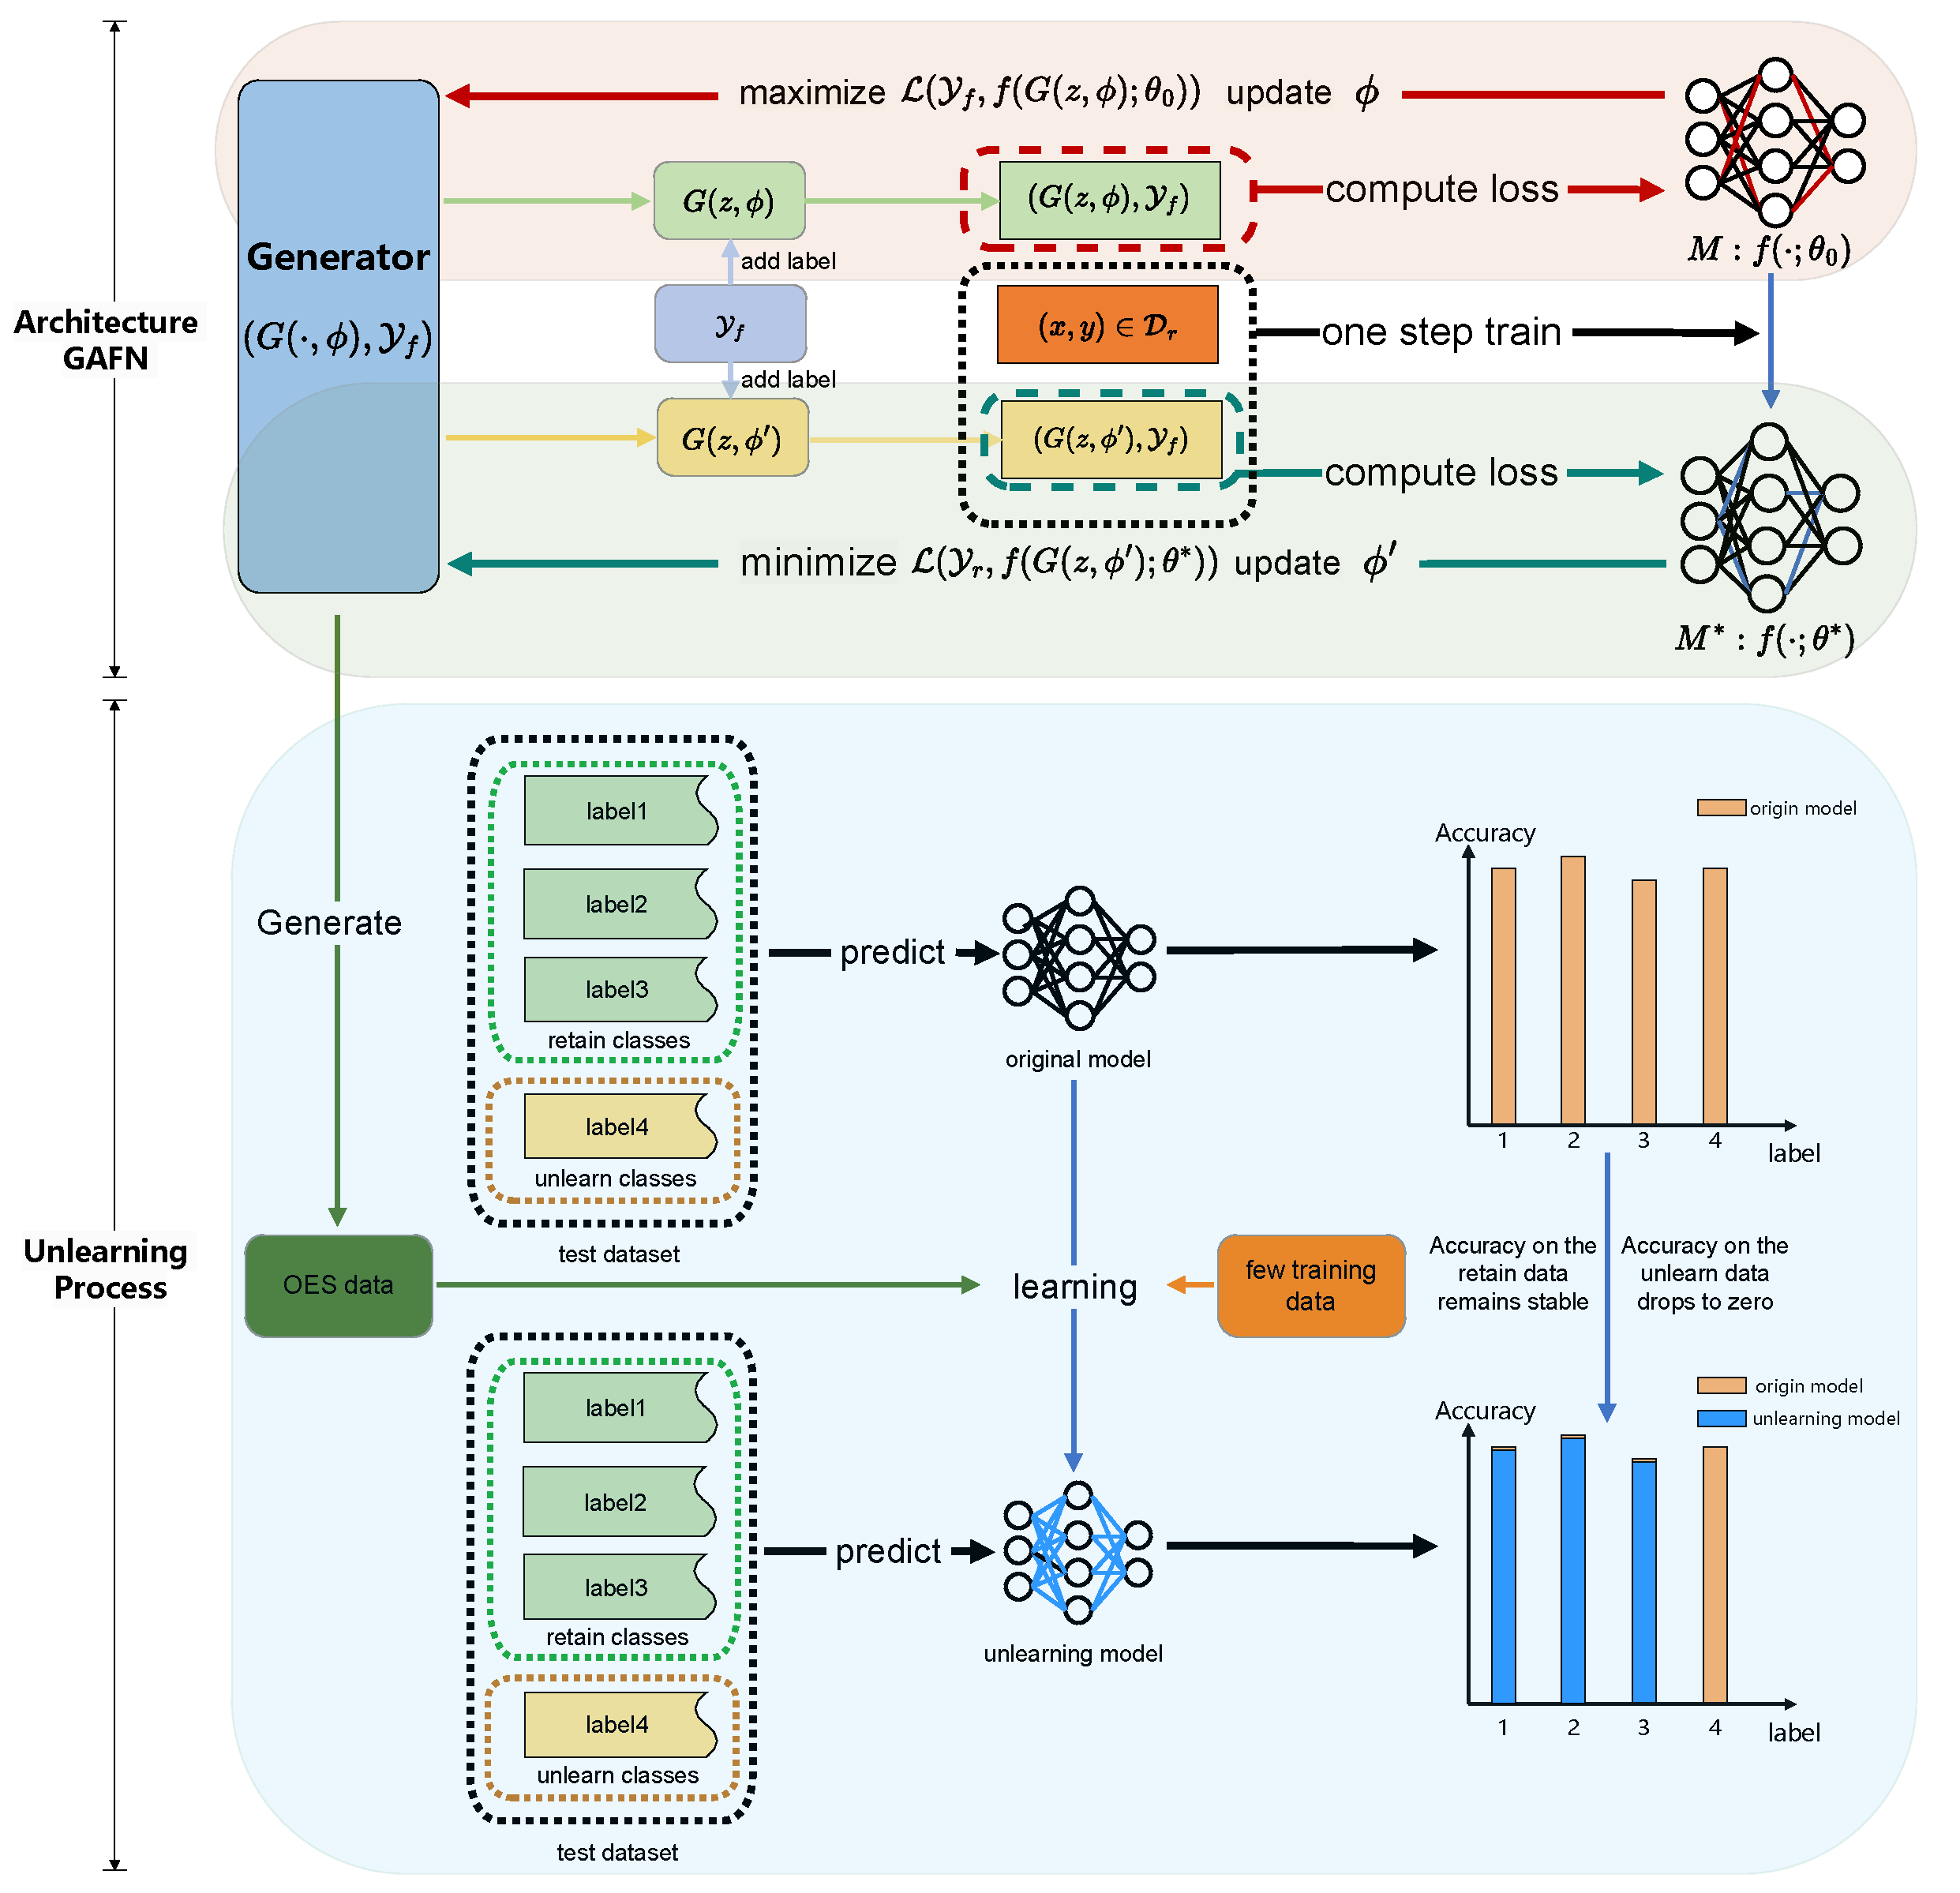
\includegraphics[width=\linewidth]{abstract.pdf}
\end{graphicalabstract}

%%Research highlights
\begin{highlights}
\item \textbf{Novel Framework.}
Proposed a novel framework for precise category unlearning under zero-glance conditions, enabling effective and secure unlearning in a few-shot scenario.

\item \textbf{Optimal Erasure Samples.}
The incremental learning strategy using the generated OES data effectively mitigates the impact of data to be forgotten on the model while maintaining performance on retained classes.
    
\item \textbf{Generative Adversarial Feedback Network.}
Developed the GAFN to generate optimal erasure samples using a portion of the training dataset, following the design principle of maximising the loss for forgotten classes while minimising the impact on retained classes.

\item \textbf{Outstanding Performance.}
Validated on public datasets, achieving state-of-the-art results in unlearning effectiveness and robustness in a few-shot scenario.

\end{highlights}

\begin{keyword}
Machine Unlearning, Incremental Learning
\end{keyword}


\end{frontmatter}

\linenumbers

\section{Introduction}

Machine learning has become integral to applications across various domains, including healthcare~\cite{shailaja2018machine}, finance~\cite{dixon2020machine}, and fairness~\cite{xu2022assessing,xu2023disentangled}, due to its ability to predict complex patterns. Uploading data to online services traditionally meant allowing providers to use it freely. However, growing awareness of data sensitivity has led to regulations, e.g., the General Data Protection Regulation (GDPR)~\cite{voigt2017eu}, the California Consumer Privacy Act (CCPA)~\cite{goldman2020introduction}, and China’s Personal Information Protection Law (PIPL)~\cite{calzada2022citizens}, which allow users more control and the “right to be forgotten”~\cite{villaronga2018humans}.



\begin{figure}[t]  
    \centering
    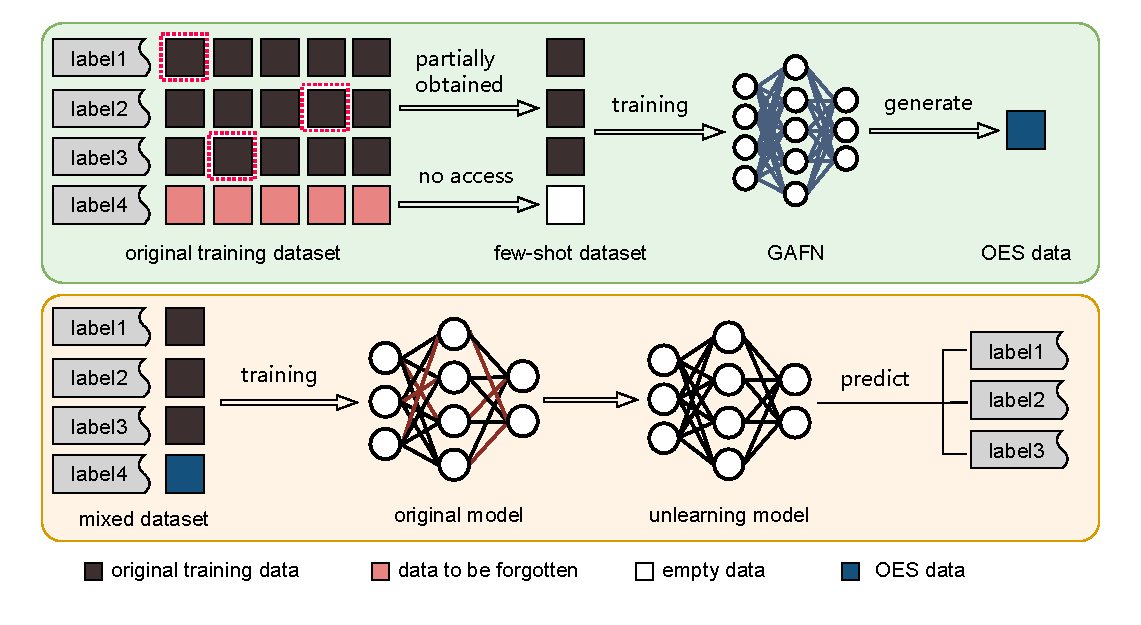
\includegraphics[width=\textwidth]{pic1.pdf}
    \caption{The training process of GAFN on the few-shot dataset to generate OES data (top), followed by incremental training of the original model using the OES data for machine unlearning (bottom).}
    \label{fig_figure1}
\end{figure}

Despite these regulations, there is a growing demand for methods to ensure the removal of private data from machine learning models without compromising performance~\cite{al2019privacy}. For example, in a healthcare scenario where a patient requests the removal of their medical records from a predictive model~\cite{miotto2018deep}, the predictive model must erase all traces of the patient's data to comply with privacy regulations while still maintaining its accuracy performance for other patients~\cite{abouelmehdi2018big}. Existing solutions, such as retraining models~\cite{wu2020deltagrad} or employing complex data handling techniques~\cite{shaik2023exploring}, are often computationally expensive and impractical, particularly in scenarios where the original training dataset is not fully accessible, a setting known as few-shot unlearning~\cite{GuoGHM20}. Moreover, current few-shot unlearning approaches face even greater challenges in zero-glance scenarios, where the data to be forgotten is completely inaccessible during the unlearning process. These methods often struggle to balance the effective removal of the targeted data’s influence with maintaining overall model performance. This is primarily due to their reliance on complex mechanisms and their inability to efficiently handle such strict data constraints. Therefore, there is a pressing need for innovative frameworks that can achieve unlearning under these restrictive conditions while ensuring computational efficiency and high predictive accuracy.


To address these challenges, we propose a machine unlearning framework based on incremental learning, designed specifically for zero-glance scenarios where the data to be forgotten is completely inaccessible. This framework utilizes \textit{Optimal Erasure Samples} (OES) and the \textit{Generative Adversarial Feedback Network} (GAFN) to achieve precise category unlearning under these strict conditions. Figure \ref{fig_figure1} illustrates the elimination of the data to be forgotten from the machine learning model in few-shot unlearning scenarios. The GAFN is trained exclusively on a small, accessible subset of the dataset and generates OES, i.e., samples that have the most significant impact on the data to be forgotten, despite having no direct access to it. These OES are then used to incrementally retrain the original predictive model, enabling effective machine unlearning. The primary goal of designing OES is to precisely remove the influence of the target data while ensuring the predictive model retains its performance on the retained data. By combining the incremental learning approach with a generative model trained under zero-glance constraints, our framework ensures precise unlearning in few-shot scenarios while balancing model effectiveness and privacy protection.

In summary, we make the following contributions:

\begin{itemize}
    \item We introduce a novel framework for machine unlearning based on incremental learning to achieve precise category unlearning in few-shot scenarios under zero-glance conditions. 
    
    \item We design the \textit{Optimal Erasure Samples} (OES) strategy to effectively erase the influence of specific data on the predictive model by maximising the loss for classes to be forgotten while minimising the loss for retained classes.
    
    \item We develop a \textit{Generative Adversarial Feedback Network} (GAFN) to generate OES data. By leveraging a small portion of the available training dataset, GAFN generates samples that result in a high loss for classes to be forgotten and minimal impact on retained classes. 
    
    \item We conduct extensive comparative experiments on publicly available datasets. The proposed framework outperforms state-of-the-art solutions in both effectiveness and maintaining the performance of the predictive model even with limited training samples. These findings highlight the practical applicability and robustness of our approach in real-world scenarios.
\end{itemize}

\section{Related Work}
In recent years, growing public awareness of the right to deletion has driven significant interest in research on machine unlearning~\cite{juliussen2023algorithms,chen2021machine,floridi2023machine}. Existing approaches to machine unlearning can be broadly categorised into two types: exact unlearning and approximate unlearning. Moreover, due to constraints in data management and strict privacy protection regulations~\cite{bygrave2010privacy}, accessing the complete training dataset during the machine learning process is often infeasible. To address this challenge, few-shot unlearning has emerged as a promising research direction within the field of machine unlearning. The following sections provide a comprehensive overview of machine unlearning, focusing on exact unlearning, approximate unlearning, and the emerging paradigm of few-shot unlearning.


\subsection{Exact unlearning}
Exact unlearning seeks to eliminate the influence of designated data instances in a machine learning model. This approach ensures that, after unlearning, the model's parameters and outputs are indistinguishable from those of a model trained without the removed data.

Exact unlearning was first studied by   Cao et al.~\cite{2015Towards}, who introduced the foundational concepts for systematically removing the influence of specific data points from machine learning models. Building on this, Ginart et al.~\cite{ginart2019making} proposed an unlearning method for the K-means clustering algorithm, leveraging quantisation and data partitioning for incremental learning. Subsequently, Ginart et al.~\cite{2021Machine} introduced the well-known SISA framework, which uses dataset sharding and multiple model training to establish a primary framework for exact unlearning. Yan et al.~\cite{yan2022arcane} further enhanced SISA by integrating a memory-augmented model, improving the efficiency of the unlearning process. Aldaghri et al.~\cite{aldaghri2021coded} improved the time efficiency of exact unlearning by encoding training data into shards using linear encoders prior to the learning phase.

Despite these advances, existing methods often mimic the retraining process and depend heavily on access to the complete training dataset. In real-world scenarios, such requirements result in higher computational costs, longer training times, and significant compliance expenses for enterprises or data controllers striving to fulfil right-to-deletion obligations.

\subsection{Approximate Unlearning}
Approximate unlearning seeks to reduce or minimise the influence of specified data points efficiently, without necessarily achieving perfect removal. This approach employs approximation techniques to make the behaviour of the model closely resemble that of a model trained without the removed data while avoiding the computational burden of full retraining.

In the study of approximate unlearning, various approaches have been proposed. Guo et al.~\cite{GuoGHM20} introduced Certified Removal, pioneering the application of Influence Functions~\cite{koh2017understanding} from statistics to machine unlearning. Izzo et al.~\cite{izzo2021approximate} proposed a linear logistic model approximation for unlearning, using projective residual updates to approximate the Hessian matrix, which is particularly effective for small sample sizes. Golatkar et al.~\cite{golatkar2021mixed} utilised the Fisher information matrix to quantify and identify key parameters in deep networks associated with training samples, enabling the retention of core data while removing non-core data, thereby enhancing the efficiency and accuracy of unlearning. Unlike retraining, these methods leverage the inherent stochasticity and incremental nature of the training process \cite{parisi2019continual,read2012batch,dohare2024loss}, but can sometimes adversely impact the performance of predictive models \cite{golatkar2020forgetting,chundawat2023can}.
Another direction of approximate unlearning focuses on adjusting predictive model parameters to eliminate the influence of data that must be forgotten \cite{golatkar2020eternal}. While these methods avoid the high costs of retraining, they may result in some loss of predictive performance \cite{golatkar2020forgetting,chundawat2023can}.


\subsection{Few-shot unlearning}
As a sub-field of approximate unlearning, few-shot unlearning methods \cite{peste2021ssse} aim to achieve unlearning by accessing only a portion of the training dataset. Among existing approaches, gradient-based adjustments that modify predictive model weights to forget specific data points represent the most straightforward strategy \cite{golatkar2020eternal}. However, these methods often incur significant computational overhead and are particularly ineffective when dealing with non-convex loss functions and complex predictive models.

To address these limitations, Golatkar et al.~\cite{golatkar2020forgetting} proposed an information-theoretic approach leveraging Neural Tangent Kernel (NTK) approximations to estimate the weight updates required for unlearning. By approximating the complex dynamics of model training, this method offers a theoretical foundation for reducing computational complexity. However, despite its promise, the NTK-based approach remains resource-intensive, suffers from accuracy degradation even in small datasets, and is challenging to scale for larger or more complex scenarios.

Building on the need for alternatives to gradient-based methods, Youngsik Yoon et al.~\cite{yoon2023fewshot}  introduced an inversion-based unlearning technique that reverses the predictive model's learning process \cite{parish2016paradigm}. This method relies on generating proxy data through model inversion to simulate the training data's removal. While this approach avoids direct gradient updates, it often leads to unstable unlearning effects, especially in contexts where strict privacy requirements or limited access to original data constrain the process.

To further enhance efficiency, Tarun et al.~\cite{tarun2023fast} proposed the Unlearning by Selective Impair and Repair (UNSIR) method. UNSIR achieves rapid unlearning by generating error-maximizing noise and applying a high learning rate to expedite the process. Compared to NTK-based and inversion-based methods, UNSIR offers significant gains in unlearning speed. However, it introduces new challenges, such as designing effective noise matrices and managing the repair steps required for multi-class unlearning tasks, which remain areas for improvement.

\subsection{Discussion}
With the rise of increasingly stringent privacy protection regulations~\cite{ausloos2012right}, few-shot unlearning has emerged as a pivotal area of research within the field of machine unlearning~\cite{liu2024survey}. Its reduced reliance on large datasets and computational resources makes it more practical for real-world applications and better suited for meeting legal compliance requirements compared to other methods.

Despite the advantages of existing few-shot unlearning techniques, they face notable challenges in terms of robustness, scalability, and effectiveness, particularly in low-data scenarios. To address these limitations, we propose a novel framework for class unlearning in few-shot scenarios, designed to operate under stricter privacy conditions, which we term zero-glance, a setting where the data to be forgotten is entirely inaccessible. Our framework demonstrates significant improvements over state-of-the-art methods in both accuracy and robustness, offering promising potential for broader applications in data-sensitive domains.

\section{Methodology}
\subsection{Preliminary}
For a given dataset $\mathcal{D}$, consisting of $\mathcal{K}$ classes with $n$ samples, i.e., $\mathcal{D} = \{(x_i, y_i)\}_{i=1}^n$, where $x_i \in \mathcal{X} \subset \mathbb{R}^d$ and $y_i \in \mathcal{Y} = \{1, \ldots, \mathcal{K}\}$, the goal of a classification problem is to learn a mapping $F: \mathcal{X} \rightarrow \mathcal{Y}$ such that $F(\mathcal{X}) = \mathcal{Y}$. Given a model \(M: f(\cdot; \theta)\) with parameters $\theta$, the optimal parameters $\theta_0$ are obtained by minimising the classification loss function $\mathcal{L}(\mathcal{Y}, f(\cdot; \theta))$ on the dataset $\mathcal{D}$.

Machine unlearning refers to remove the influence of a specific subset of data, $\mathcal{D}_f \subseteq \mathcal{D}$, from a trained model. The most straightforward solution is to retrain a new predictive model on the remaining dataset $\mathcal{D} \setminus \mathcal{D}_f$. However, this method requires access to the entire dataset $\mathcal{D}$, which is often impractical due to privacy concerns, or data access limitations.

In a few-shot unlearning scenario, only a subset $\mathcal{D}_s \subseteq \mathcal{D}$ is accessible. The goal is to mitigate the impact of $\mathcal{D}_f$ on the model while maintaining the predictive model's performance. Let $\mathcal{Y}_f$ be the labels of classes to be forgotten and $\mathcal{Y}_r$ be the labels of classes to be retained, where $\mathcal{Y}_f \cap \mathcal{Y}_r = \emptyset$ and $\mathcal{Y}_f \cup \mathcal{Y}_r = \mathcal{Y}$. The corresponding sample sets $\mathcal{D}_f$ and $\mathcal{D}_r$ satisfy $\mathcal{D}_f \cap \mathcal{D}_r = \emptyset$ and $\mathcal{D}_f \cup \mathcal{D}_r = \mathcal{D}_s$. 

\subsection{Optimal Erasure Samples}

% \input{Figures/figure2}

\begin{figure}[t]  % 't' option places the figure at the top of the page
    \centering
    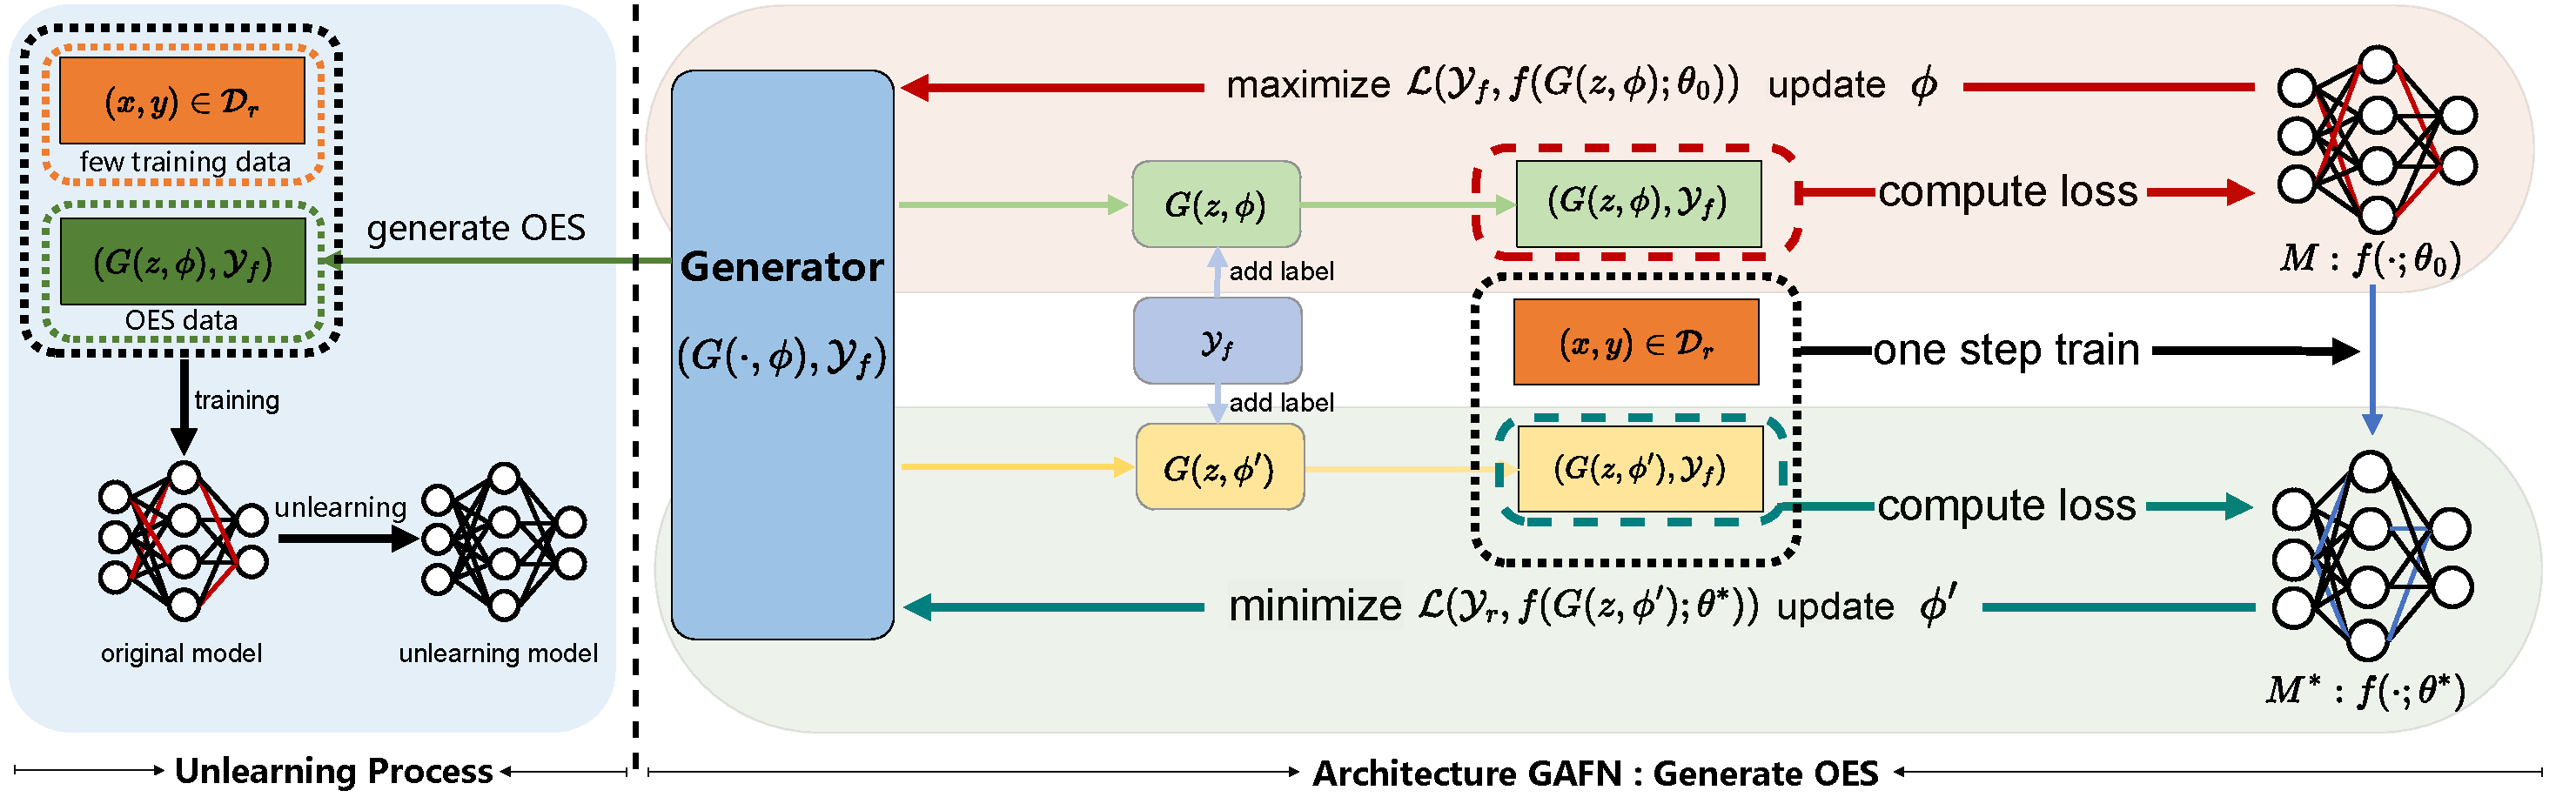
\includegraphics[width=\textwidth]{pic2.pdf}
    \caption{The architecture of GAFN consists of two parts: the \textit{Maximise} part (light pink bottom part) and the \textit{Minimise} part (light green bottom part) for generating OES data, as shown on the right side. The left side illustrates the process of machine unlearning training on OES data. }
    \label{fig_figure2}
\end{figure}

The purpose of \textit{Optimal Erasure Samples} (OES) is to enable the predictive model to precisely eliminate the influence of the data to be forgotten after incremental learning. In the few-shot scenario, OES must meet the following criteria:

\begin{enumerate}
  \item OES labelled as $\mathcal{Y}_f$ should have a large classification loss on the original predictive model.
  \item The predictive model trained with OES data should have a small classification loss on the retain data, ideally consistent with the classification loss before incremental learning.
\end{enumerate}

Based on the above criteria, we provide a formal definition of OES as follows:

\begin{definition}[Optimal Erasure Samples (OES)]
    The samples in dataset \( \mathcal{D}_j^* = \{(x_i^*, y_{j})\}_{i=1}^s \) are defined as OES if it satisfies the following conditions for \( y_{j} \in \mathcal{Y}_f \):
    \begin{align}
    \mathcal{D}_j^* = \arg\max_{\mathcal{D}_j^*} \frac{1}{s} \sum_{i=1}^{s} \mathcal{L}(y_{j}, f({x_i}^*; \theta)), \label{eq1}
    \end{align}
    \begin{align}
    \begin{split}
    |\mathcal{L}(\mathcal{Y}_{r}, f(\cdot; \theta^*)) - \mathcal{L}(\mathcal{Y}, f(\cdot; \theta))| \leq ~~~~~~~~~~~~~~~\\
    \epsilon \cdot \max(|\mathcal{L}(\mathcal{Y}_{r}, f(\cdot; \theta^*))|, |\mathcal{L}(\mathcal{Y}, f(\cdot; \theta))|), \label{eq2}
    \end{split}
    \end{align}
    \begin{align}
    \theta^* = \arg\min_{\theta} \frac{1}{s} \sum_{i=1}^{s} \mathcal{L}(y_{j}, f({x_i}^*; \theta)). \label{eq3}
    \end{align}
\end{definition}

Equation \ref{eq1} ensures that OES labelled as $\mathcal{Y}_f$ has a large classification loss on the original predictive model, maximising the influence on the classes to be forgotten. Equations \ref{eq2} and \ref{eq3} measure the predictive model's performance on the retain data before and after learning the OES. We define $\epsilon$ as a \textit{impact factor}, indicating how close the classification loss on retain data remains to the original predictive model. A smaller value of $\epsilon$ indicates that the predictive model's classification loss on retain data is more consistent with the original predictive model, thereby ensuring minimal impact on retain classes.

\subsection{Generative Adversarial Feedback Network}

In this section, we introduce the \textit{Generative Adversarial Feedback Network} (GAFN), which is designed to generate OES for precise unlearning in few-shot scenarios. We begin by explaining the need for the neural network, followed by a detailed explanation of the proposed GAFN’s architecture.

% \input{algorithms/algorithm1}

\begin{algorithm}[h]
\caption{Optimal Erasure Samples (OES) Generation using GAFN}
\begin{algorithmic}[1]
\STATE \textbf{Input:}  $\mathcal{D}$, $M$ ,$\theta$, $\mathcal{Y}_f$, $\mathcal{D}_s$,  $\alpha$
\STATE \textbf{Output:} $G$ (params: $\phi^*$)

\STATE Initialize $G$ with parameters $\phi$ and random noise $z$
\STATE Train $G$ to generate OES:

\STATE \quad \textbf{Maximize Part:}
\STATE \quad \quad (a) Fix $M$ parameters $\theta_0$
\STATE \quad \quad (b) Generate samples $G(z, \phi)$ with labels $\mathcal{Y}_f$
\STATE \quad \quad (c) Compute $\mathcal{L}(\mathcal{Y}_f, f(G(z, \phi); \theta_0))$ and maximize w.r.t. $\phi$:
\[
\phi' = \phi - \alpha \nabla_\phi \left(-\mathcal{L}(\mathcal{Y}_f, f(G(z, \phi); \theta_0))\right)
\]
\STATE \quad \quad (d) Update $M$ with $G(z, \phi')$ and $\mathcal{D}_r$ (one training step):
\[
\theta^* = \theta_0 - \alpha \nabla_\theta \mathcal{L}(\mathcal{Y}_f \cup \mathcal{Y}_r, f(G(z, \phi); \theta_0))
\]

\STATE \quad \textbf{Minimize Part:}
\STATE \quad \quad (a) Fix updated $M$ parameters $\theta^*$
\STATE \quad \quad (b) Use $\mathcal{D}_r$ to minimize loss, updating $\phi$:
\[
\phi^* = \phi' - \alpha \nabla_\phi \mathcal{L}(\mathcal{Y}_r, f(x_r; \theta^*))
\]

\RETURN $G$ (params: $\phi^*$)
\end{algorithmic}
\end{algorithm}


We note that directly solving for OES presents significant challenges. First, non-linearity, complex constraints, high dimensionality of the optimization problem, and reliance on gradient information make direct OES generation difficult. Additionally, during the OES generation process, we must ensure zero-glance, which means that we cannot use any data that needs to be forgotten.

To overcome these challenges, we implement two key strategies. First, we construct a generative network model that transforms the complex OES problem into a neural network training task. By leveraging adversarial generation techniques, this approach enables the creation of OES that allows the predictive model to forget specific classes while preserving its performance on others. Second, we employ Complement Set Inference, which indirectly trains the GAFN using the complement set of the data slated for deletion from a small training dataset. This involves generating new labelled data for the classes requiring forgotten, ensuring they induce a large loss on the original predictive model. Feedback from the small training dataset is then used to fine-tune the generated data, which allows precise interference while maintaining the predictive model’s overall performance.

The architecture of GAFN is shown in the \textit{right} of Figure~\ref{fig_figure2}, GAFN is composed of two primary components: the \textit{Maximise} part and the \textit{Minimise} part. The generator \(G(\cdot, \phi)\) is initialised and provided with random noise \(z\). The objective is to train the generator \(G\) using both components to generate OES.

The \textit{Maximise} part is highlighted in light pink in Figure~\ref{fig_figure2}. The original predictive model $M$: $f(\cdot; \theta_0)$ accepts samples generated by the generator \(G(z, \phi)\) and uses the classes \(\mathcal{Y}_f\) that need to be forgotten as labels. By fixing the parameters of predictive model $M$, we compute the loss function \(\mathcal{L}(\mathcal{Y}_f, f(G(z, \phi); \theta_0))\). This loss function is maximised through back-propagation to update the generator \(G\):
\begin{equation}
\phi' = \phi - \alpha \nabla_\phi \left(-\mathcal{L}(\mathcal{Y}_f, f(G(z, \phi); \theta_0))\right).
\end{equation}

The goal is to maximise the loss of the original predictive model on generated samples with labels of the classes to be forgotten, rapidly disrupting the features learned by the predictive model about \( \mathcal{Y}_f \). After updating the generator \(G\), the predictive model is provided with these generated samples \((G(z, \phi'), \mathcal{Y}_f)\) along with a partial training dataset \( \mathcal{D}_r \) for one step of training. During this process, the predictive model \(M: f(\cdot; \theta_0)\) is updated using:

\begin{equation}
\theta^* = \theta_0 - \alpha \nabla_\theta \mathcal{L}(\mathcal{Y}_f \cup \mathcal{Y}_r, f(G(z, \phi); \theta_0)).
\end{equation}

To mitigate the impact on the retain data, we then proceed with the \textit{Minimise} part.

The \textit{Minimise} part is highlighted in light green in Figure~\ref{fig_figure2}, and aims to eliminate the decrease in predictive model accuracy caused by the parameter updates in the \textit{Maximise} part. Based on the dataset $\mathcal{D}_r$, we train the generator \(G\) again, and fix the parameters \(\theta^*\). From the \textit{Maximise} part,  we note that \(\theta^*\) is a function of \(\phi\), denoted as \(\theta^* = \sigma(\phi)\). The loss function \(\mathcal{L}(\mathcal{Y}_r, f(x_r; \theta^*))\) is computed and minimised through back-propagation to update the generator \(G\):
\begin{equation}
\phi^* = \phi' - \alpha \nabla_\phi \mathcal{L}(\mathcal{Y}_r, f(x_r; \theta^*)).
\end{equation}

According to the chain rule of gradient computation, this formula can be further processed as:
\begin{equation}
\phi^* = \phi' - \alpha \nabla_\theta \mathcal{L}(\mathcal{Y}_r, f(x_r; \theta^*)) \cdot \nabla_\phi \sigma(\phi).
\end{equation}

The training algorithm for the generator \(G\) is presented as Algorithm 1. The generator \(G\) is initially trained using the \textit{Maximise} part to generate samples labelled as \(\mathcal{Y}_f\). Then, the generated samples are refined using the \textit{Minimise} part to eliminate any influence on the retain data. By alternately training the generator \(G\), we ensure that the generated samples precisely mitigate the impact of the classes to be forgotten during the incremental learning process of the original model, while minimising the effect on the predictive performance of the model.

\begin{algorithm}[h]
\caption{Incremental Learning Strategy for Unlearning and Enhancement}
\begin{algorithmic}[1]
\STATE \textbf{Input:}  $\mathcal{D}$,  $M$ ,$\theta_0$, $G$ ,$\phi^*$, Retain classes $\mathcal{Y}_r$, $\mathcal{Y}_f$,  $\alpha$
\STATE \textbf{Output:}  $M$ (params: $\theta^*$)

\STATE Initialize $M$ with parameters $\theta_0$ and $G$ with $\phi^*$
\STATE Train $M$ to unlearn classes $\mathcal{Y}_f$:

\STATE \quad \textbf{Unlearning Process:}
\STATE \quad \quad (a) Fix $G$ parameters $\phi^*$
\STATE \quad \quad (b) Generate samples $G(z, \phi^*)$ with labels $\mathcal{Y}_f$
\STATE \quad \quad (c) Compute $\mathcal{L}(\mathcal{Y}_f, f(G(z, \phi^*); \theta_0))$ and minimize w.r.t. $\theta$:
\[
\theta' = \theta_0 - \alpha \nabla_\theta \mathcal{L}(\mathcal{Y}_f, f(G(z, \phi^*); \theta_0))
\]

\STATE \quad \textbf{Enhancement Process:}
\STATE \quad \quad (a) Fix updated $M$ parameters $\theta'$
\STATE \quad \quad (b) Use retain data $\mathcal{D}_r$ to improve performance on $\mathcal{Y}_r$:
\[
\theta^* = \theta' - \alpha \nabla_\theta \mathcal{L}(\mathcal{Y}_r, f(x_r; \theta'))
\]

\RETURN $M$ (params: $\theta^*$)
\end{algorithmic}
\end{algorithm}


\subsection{Incremental learning Strategy}

We present the algorithm for using OES in incremental learning to achieve unlearning, as shown in Algorithm 2 above. To achieve precise unlearning while preserving the original performance of the predictive model, we build upon the OES generated by GAFN and further propose the following incremental learning strategies:

\begin{itemize}
  \item \textbf{Collaborative Training:} In our framework, unlearning objectives and the performance of the predictive model are equally important. The best practice is to include an equal amount of OES and a small portion of the training dataset in each batch and feed them into the predictive model. This balanced practice ensures that the predictive model does not overemphasise any specific type of data during training.

  \item \textbf{Learning Rate Adjustment:} The learning rate during the incremental learning phase should not be the same as the one used during the initial training of the predictive model. Generally, it should be slightly higher, but not by several orders of magnitude. This adjustment allows the predictive model to effectively adapt its parameters during the unlearning process to accommodate the high loss associated with OES on the classes to be forgotten.

  \item \textbf{Optional Reinforcement Phase:} An optional reinforcement phase involves using a small portion of the training dataset to slightly enhance the predictive model after unlearning. This helps improve the predictive model's performance on the retain data. The decision to include this phase depends on the quality of the OES and the overall performance of the predictive model after unlearning.
\end{itemize}

Our framework employs the GAFN to generate OES for precise unlearning. By leveraging these sophisticated strategies, our incremental machine unlearning method ensures that the predictive model can forget specified data while retaining its predictive capabilities on the retain data.

\section{Experiment}

\subsection{Experimental Setup and Evaluation Metrics}
\label{subsec_experiment_setup}

\subsubsection{Datasets}  
We select three datasets for our experiments: Fashion MNIST ~\cite{xiao2017fashion}, CIFAR-10, and CIFAR-20~\cite{krizhevsky2009learning}. In all experiments, we assume that a portion of the original training dataset is uniformly distributed in each class. We set the parameter $e$ to represent the sample proportion in the original training dataset for each class, with $e=20\%$. We apply unlearning to 1, 2, 4, and 7 classes from the predictive models.


\subsubsection{Predictive Models}
The experiments involve two different predictive models: (1) AllCNN ~\cite{springenberg2014striving}, a fully connected network featuring nine convolutional layers with ReLU activation functions, followed by an adaptive average pooling layer. The original predictive model is trained with a batch size of 256 using the Adam optimiser at a learning rate of 0.0004 for 40 epochs. (2) ResNet18~\cite{he2016deep}, a residual network with skip connections to aid in training deeper networks. The original predictive model is trained with a batch size of 256 using the Adam optimizer at a learning rate of 0.0004 for 40 epochs. A weight decay of $1 \times 10^{-4}$ is introduced.



\subsubsection{Baselines}
We select the following classical~\cite{golatkar2020eternal}and state-of-the-art machine unlearning algorithms~\cite{golatkar2020eternal}~\cite{yoon2022few}~\cite{fastchundawat2023zero}~\cite{tarun2023fast}in the few-shot scenario as our comparison targets. It is important to note that, for the baseline methods, we strictly provide sufficient conditions according to the requirements of the algorithms themselves. Moreover, we do not impose restrictions on their access to the training dataset or require dataset integrity. Our goal is to enable these comparison algorithms to achieve their best performance and demonstrate the advantages of our framework by comparing it against their optimal results.
\begin{itemize}
    \item  CRetrain~\cite{nguyen2022survey}: Training a new model from scratch using only the retain data, serves as the benchmark gold standard for machine unlearning evaluations. We denote it as CRetrain.
    \item  Finetune~\cite{golatkar2020eternal}: Fine-tuning the original model on the  with a slightly increased learning rate induces forgetting of the forget data.
    \item  NegGrad~\cite{golatkar2020eternal}: Fine-tuning the original model on forget data by moving in the direction of increasing loss.
    % achieves efficient training and effective forgetting.
    \item  RL~\cite{golatkar2020eternal}: Replacing the labels of retain data with random labels and then fine-tuning on both retain data and  forget data.
    % provides a simple approach that simultaneously achieves forgetting and performance retention.
    \item  MI~\cite{yoon2022few}: Using model inversion to generate a proxy dataset, this method fine-tunes the original model, inducing targeted forgetting through weight updates.
    % Using model inversion to create a proxy dataset, this method fine-tunes the original model, strategically inducing forgetting of  forget data through intentional weight updates aligned with unlearning goals, such as privacy protection or label correction.
    \item  GKT~\cite{fastchundawat2023zero} Using adversarial pseudo-data, this method fine-tunes the original model to filter out forget data, achieving class-specific forgetting through controlled knowledge transfer. 
    \item  UNSIR~\cite{tarun2023fast}: Using error-maximising noise, this method induces forgetting by impairing weights tied to forget data, then repairs to recover accuracy on retain data, representing the state-of-the-art in few-shot unlearning.
\end{itemize}

\subsubsection{Evaluation Metrics}

Machine unlearning is still an emerging field, and there are currently no systematic and comprehensive evaluation metrics~\cite{zhang2023review}. The metrics proposed by existing unlearning algorithms are often designed for their specific scenarios. For example, in classification tasks, the prediction accuracy for the forgotten classes is a key reference metric. Therefore, we conducted a thorough evaluation of the forgetting performance of our proposed framework by combining our algorithm’s specific scenario with established methodologies from studies in the few-shot unlearning domain. We referred to existing works~\cite{nguyen2022survey,golatkar2020eternal,yoon2022few,fastchundawat2023zero,tarun2023fast} to comprehensively evaluate the effectiveness of our framework and selected the following targeted metrics:

% % \begin{table*}[t]
% \centering
% \small
% \setlength{\aboverulesep}{0pt}
% \setlength{\belowrulesep}{0pt}
% \setlength{\extrarowheight}{0.3pt} % 调整行高
% \begin{tabular}{c|cr|ccccccccc}
% \toprule
% \multirow{2.5}{*}{Models} & \multirow{2.5}{*}{$\#\mathcal{Y}_f$} & \multirow{2.5}{*}{Metrics} & \multicolumn{9}{c}{\textbf{Fashion MNIST}} \\
% \cmidrule(lr){4-12}
%  & & & Original & CRetrain & Finetune & NegGrad & RL & MI & GKT & UNSIR & \textbf{Ours} \\
% \midrule

% \multirow{12}{*}{\rotatebox{90}{\textbf{AllCNN}}}
%  & \multirow{3}{*}{1} & $A\mathcal{D}_r(\%)\uparrow$ & 90.12 & 92.36 & 90.72 & 46.58 & 85.12 & 86.13 & 81.23 & 82.50 & \underline{\textbf{88.74}} \\
%  & & $A\mathcal{D}_f(\%)\downarrow$ & 88.56 & 0.00 & 34.56 & 1.12 & 12.34 & 0.67 & 0.00 & 0.00 & \textbf{0.00} \\
%  & & $\ \ \ \ RT\ \ \ \ \ \uparrow$ & -- & \(>100\) & 27 & 45 & \(>100\) & \(>100\) & \(>100\) & \(>100\) & \(>100\) \\
% \cmidrule(lr){2-12}
%  & \multirow{3}{*}{2} & $A\mathcal{D}_r(\%)\uparrow$ & 89.47 & 93.12 & 90.14 & 50.17 & 84.47 & 85.13 & 77.54 & 78.90 & \underline{\textbf{88.65}} \\
%  & & $A\mathcal{D}_f(\%)\downarrow$ & 90.14 & 0.00 & 37.56 & 1.55 & 13.28 & 1.43 & 0.00 & 0.00 & \textbf{0.00} \\
%  & & $\ \ \ \ RT\ \ \ \ \ \uparrow$ & -- & \(>100\) & 16 & 76 & \(>100\) & \(>100\) & \(>100\) & \(>100\) & \(>100\) \\
% \cmidrule(lr){2-12}
%  & \multirow{3}{*}{4} & $A\mathcal{D}_r(\%)\uparrow$ & 88.75 & 93.20 & 88.96 & 40.27 & 83.75 & 84.21 & 74.32 & 75.90 & \underline{\textbf{90.45}} \\
%  & & $A\mathcal{D}_f(\%)\downarrow$ & 91.32 & 0.00 & 40.94 & 1.89 & 14.05 & 0.82 & 0.00 & 0.00 & \textbf{0.00} \\
%  & & $\ \ \ \ RT\ \ \ \ \ \uparrow$ & -- & \(>100\) & 21 & 33 & \(>100\) & \(>100\) & \(>100\) & \(>100\) & \(>100\) \\
% \cmidrule(lr){2-12}
%  & \multirow{3}{*}{7} & $A\mathcal{D}_r(\%)\uparrow$ & 92.14 & 95.41 & 92.41 & 50.34 & 87.34 & 88.65 & 83.12 & 84.65 & \underline{\textbf{93.12}} \\
%  & & $A\mathcal{D}_f(\%)\downarrow$ & 89.01 & 0.00 & 33.23 & 1.62 & 13.56 & 2.34 & 0.00 & 0.00 & \textbf{0.00} \\
%  & & $\ \ \ \ RT\ \ \ \ \ \uparrow$ & -- & \(>100\) & 23 & 48 & \(>100\) & \(>100\) & \(>100\) & \(>100\) & \(>100\) \\
% \midrule
% \multirow{12}{*}{\rotatebox{90}{\textbf{ResNet18}}}
%  & \multirow{3}{*}{1} & $A\mathcal{D}_r(\%)\uparrow$ & 91.23 & 93.41 & 91.76 & 54.82 & 86.23 & 87.14 & 82.67 & 83.10 & \underline{\textbf{90.34}} \\
%  & & $A\mathcal{D}_f(\%)\downarrow$ & 87.45 & 0.00 & 41.38 & 0.91 & 14.12 & 1.24 & 0.00 & 0.00 & \textbf{0.00} \\
%  & & $\ \ \ \ RT\ \ \ \ \ \uparrow$ & -- & \(>100\) & 18 & 72 & \(>100\) & \(>100\) & \(>100\) & \(>100\) & \(>100\) \\
% \cmidrule(lr){2-12}
%  & \multirow{3}{*}{2} & $A\mathcal{D}_r(\%)\uparrow$ & 89.87 & 94.85 & 89.05 & 40.98 & 85.12 & 86.13 & 75.54 & 77.32 & \underline{\textbf{90.23}} \\
%  & & $A\mathcal{D}_f(\%)\downarrow$ & 88.56 & 0.00 & 47.79 & 1.36 & 13.95 & 0.95 & 0.00 & 0.00 & \textbf{0.00} \\
%  & & $\ \ \ \ RT\ \ \ \ \ \uparrow$ & -- & \(>100\) & 27 & 66 & \(>100\) & \(>100\) & \(>100\) & \(>100\) & \(>100\) \\
% \cmidrule(lr){2-12}
%  & \multirow{3}{*}{4} & $A\mathcal{D}_r(\%)\uparrow$ & 90.54 & 92.76 & 90.79 & 30.34 & 86.12 & 85.23 & 80.54 & 81.30 & \underline{\textbf{91.45}} \\
%  & & $A\mathcal{D}_f(\%)\downarrow$ & 87.65 & 0.00 & 37.92 & 1.43 & 12.78 & 1.67 & 0.00 & 0.00 & \textbf{0.00} \\
%  & & $\ \ \ \ RT\ \ \ \ \ \uparrow$ & -- & \(>100\) & 22 & 53 & \(>100\) & \(>100\) & \(>100\) & \(>100\) & \(>100\) \\
% \cmidrule(lr){2-12}
%  & \multirow{3}{*}{7} & $A\mathcal{D}_r(\%)\uparrow$ & 93.12 & 95.34 & 92.31 & 45.73 & 89.24 & 88.15 & 83.54 & 85.10 & \underline{\textbf{94.67}} \\
%  & & $A\mathcal{D}_f(\%)\downarrow$ & 85.87 & 0.00 & 31.02 & 1.68 & 13.34 & 1.32 & 0.00 & 0.00 & \textbf{0.00} \\
%  & & $\ \ \ \ RT\ \ \ \ \ \uparrow$ & -- & \(>100\) & 14 & 29 & \(>100\) & \(>100\) & \(>100\) & \(>100\) & \(>100\) \\
% \bottomrule
% \end{tabular}
% \caption{Results of $A\mathcal{D}_r$, $A\mathcal{D}_f$, and $RT$ across different $\#\mathcal{Y}_f$ values using AllCNN and ResNet18 predictive models on Fashion MNIST datasets. The upward arrow ($\uparrow$) indicates that higher values are better, while the downward arrow ($\downarrow$) indicates that lower values are better. Underlined Values denote results within 5\% of the original predictive model's performance, and Bolded Values indicate that our framework's results differ from the CRetrain by less than 5\%.}
% \label{table_fashion_mnist}
% \end{table*}

\begin{table*}[t]
\centering
\small
\setlength{\aboverulesep}{0pt}
\setlength{\belowrulesep}{0pt}
\setlength{\extrarowheight}{0.3pt} % 调整行高
\resizebox{\textwidth}{!}{ % 调整表格宽度为页面宽度
\begin{tabular}{c|cr|ccccccccc}
\toprule
\multirow{2.5}{*}{Models} & \multirow{2.5}{*}{$\#\mathcal{Y}_f$} & \multirow{2.5}{*}{Metrics} & \multicolumn{9}{c}{\textbf{Fashion MNIST}} \\
\cmidrule(lr){4-12}
 & & & Original & CRetrain & Finetune & NegGrad & RL & MI & GKT & UNSIR & \textbf{Ours} \\
\midrule

\multirow{12}{*}{\rotatebox{90}{\textbf{AllCNN}}}
 & \multirow{3}{*}{1} & $A\mathcal{D}_r(\%)\uparrow$ & 90.12 & 92.36 & 90.72 & 46.58 & 85.12 & 86.13 & 81.23 & 82.50 & \underline{\textbf{88.74}} \\
 & & $A\mathcal{D}_f(\%)\downarrow$ & 88.56 & 0.00 & 34.56 & 1.12 & 12.34 & 0.67 & 0.00 & 0.00 & \textbf{0.00} \\
 & & $\ \ \ \ RT\ \ \ \ \ \uparrow$ & -- & \(>100\) & 27 & 45 & \(>100\) & \(>100\) & \(>100\) & \(>100\) & \(>100\) \\
\cmidrule(lr){2-12}
 & \multirow{3}{*}{2} & $A\mathcal{D}_r(\%)\uparrow$ & 89.47 & 93.12 & 90.14 & 50.17 & 84.47 & 85.13 & 77.54 & 78.90 & \underline{\textbf{88.65}} \\
 & & $A\mathcal{D}_f(\%)\downarrow$ & 90.14 & 0.00 & 37.56 & 1.55 & 13.28 & 1.43 & 0.00 & 0.00 & \textbf{0.00} \\
 & & $\ \ \ \ RT\ \ \ \ \ \uparrow$ & -- & \(>100\) & 16 & 76 & \(>100\) & \(>100\) & \(>100\) & \(>100\) & \(>100\) \\
\cmidrule(lr){2-12}
 & \multirow{3}{*}{4} & $A\mathcal{D}_r(\%)\uparrow$ & 88.75 & 93.20 & 88.96 & 40.27 & 83.75 & 84.21 & 74.32 & 75.90 & \underline{\textbf{90.45}} \\
 & & $A\mathcal{D}_f(\%)\downarrow$ & 91.32 & 0.00 & 40.94 & 1.89 & 14.05 & 0.82 & 0.00 & 0.00 & \textbf{0.00} \\
 & & $\ \ \ \ RT\ \ \ \ \ \uparrow$ & -- & \(>100\) & 21 & 33 & \(>100\) & \(>100\) & \(>100\) & \(>100\) & \(>100\) \\
\cmidrule(lr){2-12}
 & \multirow{3}{*}{7} & $A\mathcal{D}_r(\%)\uparrow$ & 92.14 & 95.41 & 92.41 & 50.34 & 87.34 & 88.65 & 83.12 & 84.65 & \underline{\textbf{93.12}} \\
 & & $A\mathcal{D}_f(\%)\downarrow$ & 89.01 & 0.00 & 33.23 & 1.62 & 13.56 & 2.34 & 0.00 & 0.00 & \textbf{0.00} \\
 & & $\ \ \ \ RT\ \ \ \ \ \uparrow$ & -- & \(>100\) & 23 & 48 & \(>100\) & \(>100\) & \(>100\) & \(>100\) & \(>100\) \\
\midrule
\multirow{12}{*}{\rotatebox{90}{\textbf{ResNet18}}}
 & \multirow{3}{*}{1} & $A\mathcal{D}_r(\%)\uparrow$ & 91.23 & 93.41 & 91.76 & 54.82 & 86.23 & 87.14 & 82.67 & 83.10 & \underline{\textbf{90.34}} \\
 & & $A\mathcal{D}_f(\%)\downarrow$ & 87.45 & 0.00 & 41.38 & 0.91 & 14.12 & 1.24 & 0.00 & 0.00 & \textbf{0.00} \\
 & & $\ \ \ \ RT\ \ \ \ \ \uparrow$ & -- & \(>100\) & 18 & 72 & \(>100\) & \(>100\) & \(>100\) & \(>100\) & \(>100\) \\
\cmidrule(lr){2-12}
 & \multirow{3}{*}{2} & $A\mathcal{D}_r(\%)\uparrow$ & 89.87 & 94.85 & 89.05 & 40.98 & 85.12 & 86.13 & 75.54 & 77.32 & \underline{\textbf{90.23}} \\
 & & $A\mathcal{D}_f(\%)\downarrow$ & 88.56 & 0.00 & 47.79 & 1.36 & 13.95 & 0.95 & 0.00 & 0.00 & \textbf{0.00} \\
 & & $\ \ \ \ RT\ \ \ \ \ \uparrow$ & -- & \(>100\) & 27 & 66 & \(>100\) & \(>100\) & \(>100\) & \(>100\) & \(>100\) \\
\cmidrule(lr){2-12}
 & \multirow{3}{*}{4} & $A\mathcal{D}_r(\%)\uparrow$ & 90.54 & 92.76 & 90.79 & 30.34 & 86.12 & 85.23 & 80.54 & 81.30 & \underline{\textbf{91.45}} \\
 & & $A\mathcal{D}_f(\%)\downarrow$ & 87.65 & 0.00 & 37.92 & 1.43 & 12.78 & 1.67 & 0.00 & 0.00 & \textbf{0.00} \\
 & & $\ \ \ \ RT\ \ \ \ \ \uparrow$ & -- & \(>100\) & 22 & 53 & \(>100\) & \(>100\) & \(>100\) & \(>100\) & \(>100\) \\
\cmidrule(lr){2-12}
 & \multirow{3}{*}{7} & $A\mathcal{D}_r(\%)\uparrow$ & 93.12 & 95.34 & 92.31 & 45.73 & 89.24 & 88.15 & 83.54 & 85.10 & \underline{\textbf{94.67}} \\
 & & $A\mathcal{D}_f(\%)\downarrow$ & 85.87 & 0.00 & 31.02 & 1.68 & 13.34 & 1.32 & 0.00 & 0.00 & \textbf{0.00} \\
 & & $\ \ \ \ RT\ \ \ \ \ \uparrow$ & -- & \(>100\) & 14 & 29 & \(>100\) & \(>100\) & \(>100\) & \(>100\) & \(>100\) \\
\bottomrule
\end{tabular}
}
\caption{Results of $A\mathcal{D}_r$, $A\mathcal{D}_f$, and $RT$ across different $\#\mathcal{Y}_f$ values using AllCNN and ResNet18 predictive models on Fashion MNIST datasets. The upward arrow ($\uparrow$) indicates that higher values are better, while the downward arrow ($\downarrow$) indicates that lower values are better. Underlined Values denote results within 5\% of the original predictive model's performance, and Bolded Values indicate that our framework's results differ from the CRetrain by less than 5\%.}
\label{table_fashion_mnist}
\end{table*}
\begin{table}[t]
\centering
\small
\setlength{\aboverulesep}{0pt}
\setlength{\belowrulesep}{0pt}
\setlength{\extrarowheight}{0.3pt} % 调整行高
\resizebox{\textwidth}{!}{ % 调整表格宽度为页面宽度
\begin{tabular}{c|cr|ccccccccc}
\toprule
\multirow{2.5}{*}{Models} & \multirow{2.5}{*}{$\#\mathcal{Y}_f$} & \multirow{2.5}{*}{Metrics} & \multicolumn{9}{c}{\textbf{Fashion MNIST}} \\
\cmidrule(lr){4-12}
 & & & Original & CRetrain & Finetune & NegGrad & RL & MI & GKT & UNSIR & \textbf{Ours} \\
\midrule

\multirow{12}{*}{\rotatebox{90}{\textbf{AllCNN}}}
 & \multirow{3}{*}{1} & $A\mathcal{D}_r(\%)\uparrow$ & 90.12 & 92.36 & 90.72 & 46.58 & 85.12 & 86.13 & 81.23 & 82.50 & \underline{\textbf{88.74}} \\
 & & $A\mathcal{D}_f(\%)\downarrow$ & 88.56 & 0.00 & 34.56 & 1.12 & 12.34 & 0.67 & 0.00 & 0.00 & \textbf{0.00} \\
 & & $\ \ \ \ RT\ \ \ \ \ \uparrow$ & -- & \(>100\) & 27 & 45 & \(>100\) & \(>100\) & \(>100\) & \(>100\) & \(>100\) \\
\cmidrule(lr){2-12}
 & \multirow{3}{*}{2} & $A\mathcal{D}_r(\%)\uparrow$ & 89.47 & 93.12 & 90.14 & 50.17 & 84.47 & 85.13 & 77.54 & 78.90 & \underline{\textbf{88.65}} \\
 & & $A\mathcal{D}_f(\%)\downarrow$ & 90.14 & 0.00 & 37.56 & 1.55 & 13.28 & 1.43 & 0.00 & 0.00 & \textbf{0.00} \\
 & & $\ \ \ \ RT\ \ \ \ \ \uparrow$ & -- & \(>100\) & 16 & 76 & \(>100\) & \(>100\) & \(>100\) & \(>100\) & \(>100\) \\
\cmidrule(lr){2-12}
 & \multirow{3}{*}{4} & $A\mathcal{D}_r(\%)\uparrow$ & 88.75 & 93.20 & 88.96 & 40.27 & 83.75 & 84.21 & 74.32 & 75.90 & \underline{\textbf{90.45}} \\
 & & $A\mathcal{D}_f(\%)\downarrow$ & 91.32 & 0.00 & 40.94 & 1.89 & 14.05 & 0.82 & 0.00 & 0.00 & \textbf{0.00} \\
 & & $\ \ \ \ RT\ \ \ \ \ \uparrow$ & -- & \(>100\) & 21 & 33 & \(>100\) & \(>100\) & \(>100\) & \(>100\) & \(>100\) \\
\cmidrule(lr){2-12}
 & \multirow{3}{*}{7} & $A\mathcal{D}_r(\%)\uparrow$ & 92.14 & 95.41 & 92.41 & 50.34 & 87.34 & 88.65 & 83.12 & 84.65 & \underline{\textbf{93.12}} \\
 & & $A\mathcal{D}_f(\%)\downarrow$ & 89.01 & 0.00 & 33.23 & 1.62 & 13.56 & 2.34 & 0.00 & 0.00 & \textbf{0.00} \\
 & & $\ \ \ \ RT\ \ \ \ \ \uparrow$ & -- & \(>100\) & 23 & 48 & \(>100\) & \(>100\) & \(>100\) & \(>100\) & \(>100\) \\
\midrule
\multirow{12}{*}{\rotatebox{90}{\textbf{ResNet18}}}
 & \multirow{3}{*}{1} & $A\mathcal{D}_r(\%)\uparrow$ & 91.23 & 93.41 & 91.76 & 54.82 & 86.23 & 87.14 & 82.67 & 83.10 & \underline{\textbf{90.34}} \\
 & & $A\mathcal{D}_f(\%)\downarrow$ & 87.45 & 0.00 & 41.38 & 0.91 & 14.12 & 1.24 & 0.00 & 0.00 & \textbf{0.00} \\
 & & $\ \ \ \ RT\ \ \ \ \ \uparrow$ & -- & \(>100\) & 18 & 72 & \(>100\) & \(>100\) & \(>100\) & \(>100\) & \(>100\) \\
\cmidrule(lr){2-12}
 & \multirow{3}{*}{2} & $A\mathcal{D}_r(\%)\uparrow$ & 89.87 & 94.85 & 89.05 & 40.98 & 85.12 & 86.13 & 75.54 & 77.32 & \underline{\textbf{90.23}} \\
 & & $A\mathcal{D}_f(\%)\downarrow$ & 88.56 & 0.00 & 47.79 & 1.36 & 13.95 & 0.95 & 0.00 & 0.00 & \textbf{0.00} \\
 & & $\ \ \ \ RT\ \ \ \ \ \uparrow$ & -- & \(>100\) & 27 & 66 & \(>100\) & \(>100\) & \(>100\) & \(>100\) & \(>100\) \\
\cmidrule(lr){2-12}
 & \multirow{3}{*}{4} & $A\mathcal{D}_r(\%)\uparrow$ & 90.54 & 92.76 & 90.79 & 30.34 & 86.12 & 85.23 & 80.54 & 81.30 & \underline{\textbf{91.45}} \\
 & & $A\mathcal{D}_f(\%)\downarrow$ & 87.65 & 0.00 & 37.92 & 1.43 & 12.78 & 1.67 & 0.00 & 0.00 & \textbf{0.00} \\
 & & $\ \ \ \ RT\ \ \ \ \ \uparrow$ & -- & \(>100\) & 22 & 53 & \(>100\) & \(>100\) & \(>100\) & \(>100\) & \(>100\) \\
\cmidrule(lr){2-12}
 & \multirow{3}{*}{7} & $A\mathcal{D}_r(\%)\uparrow$ & 93.12 & 95.34 & 92.31 & 45.73 & 89.24 & 88.15 & 83.54 & 85.10 & \underline{\textbf{94.67}} \\
 & & $A\mathcal{D}_f(\%)\downarrow$ & 85.87 & 0.00 & 31.02 & 1.68 & 13.34 & 1.32 & 0.00 & 0.00 & \textbf{0.00} \\
 & & $\ \ \ \ RT\ \ \ \ \ \uparrow$ & -- & \(>100\) & 14 & 29 & \(>100\) & \(>100\) & \(>100\) & \(>100\) & \(>100\) \\
\bottomrule
\end{tabular}
}
\caption{Results of $A\mathcal{D}_r$, $A\mathcal{D}_f$, and $RT$ across different $\#\mathcal{Y}_f$ values using AllCNN and ResNet18 predictive models on Fashion MNIST datasets. The upward arrow ($\uparrow$) indicates that higher values are better, while the downward arrow ($\downarrow$) indicates that lower values are better. Underlined Values denote results within 5\% of the original predictive model's performance, and Bolded Values indicate that our framework's results differ from the CRetrain by less than 5\%.}
\label{table_fashion_mnist}
\end{table}


% \begin{table*}[!h]
\centering
\small
\setlength{\aboverulesep}{0pt}
\setlength{\belowrulesep}{0pt}
\setlength{\extrarowheight}{0.3pt} % 调整行高
\resizebox{\textwidth}{!}{
\begin{tabular}{c|cr|ccccccccc}
\toprule
\multirow{2.5}{*}{Models} & \multirow{2.5}{*}{$\#\mathcal{Y}_f$} & \multirow{2.5}{*}{Metrics} & \multicolumn{9}{c}{\textbf{CIFAR-10}} \\
\cmidrule(lr){4-12}
 & & & Original & CRetrain & Finetune & NegGrad & RL & MI & GKT & UNSIR & \textbf{Ours} \\
\midrule
\multirow{12}{*}{\rotatebox{90}{\textbf{AllCNN}}}
 & \multirow{3}{*}{1} & $A\mathcal{D}_r(\%)\uparrow$ & 82.44 & 84.42 & 82.96 & 46.98 & 78.12 & 77.23 & 71.23 & 72.82 & \underline{\textbf{81.30}} \\
 & & $A\mathcal{D}_f(\%)\downarrow$ & 68.85 & 0.00 & 22.85 & 1.88 & 13.42 & 0.86 & 0.00 & 0.00 & \textbf{0.00} \\
 & & $\ \ \ \ RT\ \ \ \ \ \uparrow$ & -- & \(>100\) & 12 & 89 & \(>100\) & \(>100\) & \(>100\) & \(>100\) & \(>100\) \\
\cmidrule(lr){2-12}
 & \multirow{3}{*}{2} & $A\mathcal{D}_r(\%)\uparrow$ & 82.99 & 86.48 & 83.97 & 33.11 & 78.35 & 77.08 & 73.54 & 74.89 & \underline{\textbf{83.20}} \\
 & & $A\mathcal{D}_f(\%)\downarrow$ & 73.29 & 0.00 & 42.21 & 0.53 & 14.76 & 1.11 & 0.00 & 0.00 & \textbf{0.00} \\
 & & $\ \ \ \ RT\ \ \ \ \ \uparrow$ & -- & \(>100\) & 26 & 57 & \(>100\) & \(>100\) & \(>100\) & \(>100\) & \(>100\) \\
\cmidrule(lr){2-12}
 & \multirow{3}{*}{4} & $A\mathcal{D}_r(\%)\uparrow$ & 86.38 & 90.31 & 88.09 & 46.13 & 82.54 & 81.14 & 76.54 & 77.41 & \underline{\textbf{87.75}} \\
 & & $A\mathcal{D}_f(\%)\downarrow$ & 73.05 & 0.00 & 35.78 & 0.72 & 13.84 & 1.84 & 0.00 & 0.00 & \textbf{0.00} \\
 & & $\ \ \ \ RT\ \ \ \ \ \uparrow$ & -- & \(>100\) & 29 & 62 & \(>100\) & \(>100\) & \(>100\) & \(>100\) & \(>100\) \\
\cmidrule(lr){2-12}
 & \multirow{3}{*}{7} & $A\mathcal{D}_r(\%)\uparrow$ & 84.51 & 88.67 & 85.15 & 34.52 & 79.14 & 80.23 & 70.23 & 71.55 & \underline{\textbf{84.09}} \\
 & & $A\mathcal{D}_f(\%)\downarrow$ & 79.62 & 0.00 & 48.54 & 1.34 & 14.27 & 1.57 & 0.00 & 0.00 & \textbf{0.00} \\
 & & $\ \ \ \ RT\ \ \ \ \ \uparrow$ & -- & \(>100\) & 15 & 97 & \(>100\) & \(>100\) & \(>100\) & \(>100\) & \(>100\) \\
\midrule
\multirow{12}{*}{\rotatebox{90}{\textbf{ResNet18}}}
 & \multirow{3}{*}{1} & $A\mathcal{D}_r(\%)\uparrow$ & 86.99 & 88.20 & 86.38 & 46.20 & 82.05 & 83.37 & 75.23 & 76.45 & \underline{\textbf{87.10}} \\
 & & $A\mathcal{D}_f(\%)\downarrow$ & 57.06 & 0.00 & 32.41 & 1.87 & 13.59 & 0.92 & 0.00 & 0.00 & \textbf{0.00} \\
 & & $\ \ \ \ RT\ \ \ \ \ \uparrow$ & -- & \(>100\) & 13 & 58 & \(>100\) & \(>100\) & \(>100\) & \(>100\) & \(>100\) \\
\cmidrule(lr){2-12}
 & \multirow{3}{*}{2} & $A\mathcal{D}_r(\%)\uparrow$ & 87.69 & 88.31 & 88.31 & 39.55 & 83.12 & 83.85 & 75.12 & 76.50 & \underline{\textbf{87.75}} \\
 & & $A\mathcal{D}_f(\%)\downarrow$ & 69.05 & 0.00 & 49.84 & 1.14 & 14.39 & 1.38 & 0.00 & 0.00 & \textbf{0.00} \\
 & & $\ \ \ \ RT\ \ \ \ \ \uparrow$ & -- & \(>100\) & 20 & 36 & \(>100\) & \(>100\) & \(>100\) & \(>100\) & \(>100\) \\
\cmidrule(lr){2-12}
 & \multirow{3}{*}{4} & $A\mathcal{D}_r(\%)\uparrow$ & 90.73 & 92.08 & 91.63 & 35.72 & 86.23 & 87.18 & 80.54 & 82.23 & \underline{\textbf{91.37}} \\
 & & $A\mathcal{D}_f(\%)\downarrow$ & 73.85 & 0.00 & 44.57 & 0.65 & 14.02 & 0.83 & 0.00 & 0.00 & \textbf{0.00} \\
 & & $\ \ \ \ RT\ \ \ \ \ \uparrow$ & -- & \(>100\) & 28 & 71 & \(>100\) & \(>100\) & \(>100\) & \(>100\) & \(>100\) \\
\cmidrule(lr){2-12}
 & \multirow{3}{*}{7} & $A\mathcal{D}_r(\%)\uparrow$ & 91.23 & 93.15 & 91.98 & 38.12 & 87.24 & 86.29 & 76.23 & 77.85 & \underline{\textbf{91.43}} \\
 & & $A\mathcal{D}_f(\%)\downarrow$ & 80.88 & 0.00 & 46.85 & 0.87 & 13.74 & 1.74 & 0.00 & 0.00 & \textbf{0.00} \\
 & & $\ \ \ \ RT\ \ \ \ \ \uparrow$ & -- & \(>100\) & 24 & 64 & \(>100\) & \(>100\) & \(>100\) & \(>100\) & \(>100\) \\
\bottomrule
\end{tabular}
}
\caption{Rusults of $A\mathcal{D}_r$, $A\mathcal{D}_f$, and $RT$ across different $\#\mathcal{Y}_f$ values using AllCNN and ResNet18 predictive models on CIFAR-10 datasets. The upward arrow ($\uparrow$) indicates that higher values are better, while the downward arrow ($\downarrow$) indicates that lower values are better. Underlined Values denote results within 5\% of the original predictive model's performance, and Bolded Values indicate that our framework's results differ from the CRetrain by less than 5\%.}
\label{table_cifar10}
\end{table*}

\begin{table}[!h]
\centering
\small
\setlength{\aboverulesep}{0pt}
\setlength{\belowrulesep}{0pt}
\setlength{\extrarowheight}{0.3pt} % 调整行高
\resizebox{\textwidth}{!}{
\begin{tabular}{c|cr|ccccccccc}
\toprule
\multirow{2.5}{*}{Models} & \multirow{2.5}{*}{$\#\mathcal{Y}_f$} & \multirow{2.5}{*}{Metrics} & \multicolumn{9}{c}{\textbf{CIFAR-10}} \\
\cmidrule(lr){4-12}
 & & & Original & CRetrain & Finetune & NegGrad & RL & MI & GKT & UNSIR & \textbf{Ours} \\
\midrule
\multirow{12}{*}{\rotatebox{90}{\textbf{AllCNN}}}
 & \multirow{3}{*}{1} & $A\mathcal{D}_r(\%)\uparrow$ & 82.44 & 84.42 & 82.96 & 46.98 & 78.12 & 77.23 & 71.23 & 72.82 & \underline{\textbf{81.30}} \\
 & & $A\mathcal{D}_f(\%)\downarrow$ & 68.85 & 0.00 & 22.85 & 1.88 & 13.42 & 0.86 & 0.00 & 0.00 & \textbf{0.00} \\
 & & $\ \ \ \ RT\ \ \ \ \ \uparrow$ & -- & \(>100\) & 12 & 89 & \(>100\) & \(>100\) & \(>100\) & \(>100\) & \(>100\) \\
\cmidrule(lr){2-12}
 & \multirow{3}{*}{2} & $A\mathcal{D}_r(\%)\uparrow$ & 82.99 & 86.48 & 83.97 & 33.11 & 78.35 & 77.08 & 73.54 & 74.89 & \underline{\textbf{83.20}} \\
 & & $A\mathcal{D}_f(\%)\downarrow$ & 73.29 & 0.00 & 42.21 & 0.53 & 14.76 & 1.11 & 0.00 & 0.00 & \textbf{0.00} \\
 & & $\ \ \ \ RT\ \ \ \ \ \uparrow$ & -- & \(>100\) & 26 & 57 & \(>100\) & \(>100\) & \(>100\) & \(>100\) & \(>100\) \\
\cmidrule(lr){2-12}
 & \multirow{3}{*}{4} & $A\mathcal{D}_r(\%)\uparrow$ & 86.38 & 90.31 & 88.09 & 46.13 & 82.54 & 81.14 & 76.54 & 77.41 & \underline{\textbf{87.75}} \\
 & & $A\mathcal{D}_f(\%)\downarrow$ & 73.05 & 0.00 & 35.78 & 0.72 & 13.84 & 1.84 & 0.00 & 0.00 & \textbf{0.00} \\
 & & $\ \ \ \ RT\ \ \ \ \ \uparrow$ & -- & \(>100\) & 29 & 62 & \(>100\) & \(>100\) & \(>100\) & \(>100\) & \(>100\) \\
\cmidrule(lr){2-12}
 & \multirow{3}{*}{7} & $A\mathcal{D}_r(\%)\uparrow$ & 84.51 & 88.67 & 85.15 & 34.52 & 79.14 & 80.23 & 70.23 & 71.55 & \underline{\textbf{84.09}} \\
 & & $A\mathcal{D}_f(\%)\downarrow$ & 79.62 & 0.00 & 48.54 & 1.34 & 14.27 & 1.57 & 0.00 & 0.00 & \textbf{0.00} \\
 & & $\ \ \ \ RT\ \ \ \ \ \uparrow$ & -- & \(>100\) & 15 & 97 & \(>100\) & \(>100\) & \(>100\) & \(>100\) & \(>100\) \\
\midrule
\multirow{12}{*}{\rotatebox{90}{\textbf{ResNet18}}}
 & \multirow{3}{*}{1} & $A\mathcal{D}_r(\%)\uparrow$ & 86.99 & 88.20 & 86.38 & 46.20 & 82.05 & 83.37 & 75.23 & 76.45 & \underline{\textbf{87.10}} \\
 & & $A\mathcal{D}_f(\%)\downarrow$ & 57.06 & 0.00 & 32.41 & 1.87 & 13.59 & 0.92 & 0.00 & 0.00 & \textbf{0.00} \\
 & & $\ \ \ \ RT\ \ \ \ \ \uparrow$ & -- & \(>100\) & 13 & 58 & \(>100\) & \(>100\) & \(>100\) & \(>100\) & \(>100\) \\
\cmidrule(lr){2-12}
 & \multirow{3}{*}{2} & $A\mathcal{D}_r(\%)\uparrow$ & 87.69 & 88.31 & 88.31 & 39.55 & 83.12 & 83.85 & 75.12 & 76.50 & \underline{\textbf{87.75}} \\
 & & $A\mathcal{D}_f(\%)\downarrow$ & 69.05 & 0.00 & 49.84 & 1.14 & 14.39 & 1.38 & 0.00 & 0.00 & \textbf{0.00} \\
 & & $\ \ \ \ RT\ \ \ \ \ \uparrow$ & -- & \(>100\) & 20 & 36 & \(>100\) & \(>100\) & \(>100\) & \(>100\) & \(>100\) \\
\cmidrule(lr){2-12}
 & \multirow{3}{*}{4} & $A\mathcal{D}_r(\%)\uparrow$ & 90.73 & 92.08 & 91.63 & 35.72 & 86.23 & 87.18 & 80.54 & 82.23 & \underline{\textbf{91.37}} \\
 & & $A\mathcal{D}_f(\%)\downarrow$ & 73.85 & 0.00 & 44.57 & 0.65 & 14.02 & 0.83 & 0.00 & 0.00 & \textbf{0.00} \\
 & & $\ \ \ \ RT\ \ \ \ \ \uparrow$ & -- & \(>100\) & 28 & 71 & \(>100\) & \(>100\) & \(>100\) & \(>100\) & \(>100\) \\
\cmidrule(lr){2-12}
 & \multirow{3}{*}{7} & $A\mathcal{D}_r(\%)\uparrow$ & 91.23 & 93.15 & 91.98 & 38.12 & 87.24 & 86.29 & 76.23 & 77.85 & \underline{\textbf{91.43}} \\
 & & $A\mathcal{D}_f(\%)\downarrow$ & 80.88 & 0.00 & 46.85 & 0.87 & 13.74 & 1.74 & 0.00 & 0.00 & \textbf{0.00} \\
 & & $\ \ \ \ RT\ \ \ \ \ \uparrow$ & -- & \(>100\) & 24 & 64 & \(>100\) & \(>100\) & \(>100\) & \(>100\) & \(>100\) \\
\bottomrule
\end{tabular}
}
\caption{Rusults of $A\mathcal{D}_r$, $A\mathcal{D}_f$, and $RT$ across different $\#\mathcal{Y}_f$ values using AllCNN and ResNet18 predictive models on CIFAR-10 datasets. The upward arrow ($\uparrow$) indicates that higher values are better, while the downward arrow ($\downarrow$) indicates that lower values are better. Underlined Values denote results within 5\% of the original predictive model's performance, and Bolded Values indicate that our framework's results differ from the CRetrain by less than 5\%.}
\label{table_cifar10}
\end{table}



% \begin{table*}[!h]
\centering
\small
\setlength{\aboverulesep}{0pt}
\setlength{\belowrulesep}{0pt}
\setlength{\extrarowheight}{0.3pt} % 调整行高
\resizebox{\textwidth}{!}{
\begin{tabular}{c|cr|ccccccccc}
\toprule
\multirow{2.5}{*}{Models} & \multirow{2.5}{*}{$\#\mathcal{Y}_f$} & \multirow{2.5}{*}{Metrics} & \multicolumn{9}{c}{\textbf{CIFAR-20}} \\
\cmidrule(lr){4-12}
 & & & Original & CRetrain & Finetune & NegGrad & RL & MI & GKT & UNSIR & \textbf{Ours} \\
\midrule
\multirow{12}{*}{\rotatebox{90}{\textbf{AllCNN}}}
 & \multirow{3}{*}{1} & $A\mathcal{D}_r(\%)\uparrow$ & 59.17 & 60.65 & 59.76 & 15.63 & 54.12 & 55.12 & 48.23 & 49.83 & \underline{\textbf{58.34}} \\
 & & $A\mathcal{D}_f(\%)\downarrow$ & 63.12 & 0.00 & 21.89 & 0.76 & 13.47 & 0.95 & 0.00 & 0.00 & \textbf{0.00} \\
 & & $\ \ \ \ RT\ \ \ \ \ \uparrow$ & -- & \(>100\) & 17 & 24 & \(>100\) & \(>100\) & \(>100\) & \(>100\) & \(>100\) \\
\cmidrule(lr){2-12}
 & \multirow{3}{*}{2} & $A\mathcal{D}_r(\%)\uparrow$ & 58.75 & 59.90 & 59.33 & 22.43 & 55.12 & 54.04 & 46.54 & 47.13 & \underline{\textbf{58.23}} \\
 & & $A\mathcal{D}_f(\%)\downarrow$ & 65.42 & 0.00 & 41.30 & 1.26 & 15.29 & 1.03 & 0.00 & 0.00 & \textbf{0.00} \\
 & & $\ \ \ \ RT\ \ \ \ \ \uparrow$ & -- & \(>100\) & 19 & 39 & \(>100\) & \(>100\) & \(>100\) & \(>100\) & \(>100\) \\
\cmidrule(lr){2-12}
 & \multirow{3}{*}{4} & $A\mathcal{D}_r(\%)\uparrow$ & 58.35 & 60.75 & 59.03 & 11.75 & 54.54 & 53.23 & 49.12 & 50.20 & \underline{\textbf{59.87}} \\
 & & $A\mathcal{D}_f(\%)\downarrow$ & 63.60 & 0.00 & 42.19 & 0.98 & 13.83 & 1.87 & 0.00 & 0.00 & \textbf{0.00} \\
 & & $\ \ \ \ RT\ \ \ \ \ \uparrow$ & -- & \(>100\) & 14 & 55 & \(>100\) & \(>100\) & \(>100\) & \(>100\) & \(>100\) \\
\cmidrule(lr){2-12}
 & \multirow{3}{*}{7} & $A\mathcal{D}_r(\%)\uparrow$ & 56.93 & 59.98 & 57.38 & 16.52 & 53.63 & 52.47 & 45.01 & 46.21 & \underline{\textbf{55.45}} \\
 & & $A\mathcal{D}_f(\%)\downarrow$ & 64.07 & 0.00 & 52.32 & 1.09 & 14.52 & 2.17 & 0.00 & 0.00 & \textbf{0.00} \\
 & & $\ \ \ \ RT\ \ \ \ \ \uparrow$ & -- & \(>100\) & 30 & 41 & \(>100\) & \(>100\) & \(>100\) & \(>100\) & \(>100\) \\
\midrule
\multirow{12}{*}{\rotatebox{90}{\textbf{ResNet18}}}
 & \multirow{3}{*}{1} & $A\mathcal{D}_r(\%)\uparrow$ & 63.49 & 63.77 & 62.85 & 16.85 & 59.12 & 58.87 & 53.45 & 54.02 & \underline{\textbf{63.45}} \\
 & & $A\mathcal{D_f}(\%)\downarrow$ & 60.42 & 0.00 & 45.29 & 1.76 & 14.88 & 1.35 & 0.00 & 0.00 & \textbf{0.00} \\
 & & $\ \ \ \ RT\ \ \ \ \ \uparrow$ & -- & \(>100\) & 25 & 44 & \(>100\) & \(>100\) & \(>100\) & \(>100\) & \(>100\) \\
\cmidrule(lr){2-12}
 & \multirow{3}{*}{2} & $A\mathcal{D}_r(\%)\uparrow$ & 63.49 & 65.60 & 64.11 & 14.67 & 59.14 & 58.25 & 50.21 & 51.73 & \underline{\textbf{64.23}} \\
 & & $A\mathcal{D_f}(\%)\downarrow$ & 62.60 & 0.00 & 52.11 & 0.55 & 13.25 & 1.43 & 0.00 & 0.00 & \textbf{0.00} \\
 & & $\ \ \ \ RT\ \ \ \ \ \uparrow$ & -- & \(>100\) & 11 & 92 & \(>100\) & \(>100\) & \(>100\) & \(>100\) & \(>100\) \\
\cmidrule(lr){2-12}
 & \multirow{3}{*}{4} & $A\mathcal{D}_r(\%)\uparrow$ & 61.88 & 62.54 & 60.91 & 18.45 & 57.23 & 56.76 & 47.34 & 48.95 & \underline{\textbf{60.12}} \\
 & & $A\mathcal{D_f}(\%)\downarrow$ & 69.56 & 0.00 & 36.14 & 1.87 & 15.12 & 2.34 & 0.00 & 0.00 & \textbf{0.00} \\
 & & $\ \ \ \ RT\ \ \ \ \ \uparrow$ & -- & \(>100\) & 10 & 37 & \(>100\) & \(>100\) & \(>100\) & \(>100\) & \(>100\) \\
\cmidrule(lr){2-12}
 & \multirow{3}{*}{7} & $A\mathcal{D}_r(\%)\uparrow$ & 60.70 & 64.21 & 60.39 & 23.88 & 56.13 & 55.05 & 48.12 & 49.80 & \underline{\textbf{61.54}} \\
 & & $A\mathcal{D_f}(\%)\downarrow$ & 68.29 & 0.00 & 57.38 & 0.99 & 13.78 & 1.78 & 0.00 & 0.00 & \textbf{0.00} \\
 & & $\ \ \ \ RT\ \ \ \ \ \uparrow$ & -- & \(>100\) & 19 & 83 & \(>100\) & \(>100\) & \(>100\) & \(>100\) & \(>100\) \\
\bottomrule
\end{tabular}
}
\caption{Rusults of $A\mathcal{D}_r$, $A\mathcal{D}_f$, and $RT$ across different $\#\mathcal{Y}_f$ values using AllCNN and ResNet18 predictive models on CIFAR-20 datasets. The upward arrow ($\uparrow$) indicates that higher values are better, while the downward arrow ($\downarrow$) indicates that lower values are better. Underlined Values denote results within 5\% of the original predictive model's performance, and Bolded Values indicate that our framework's results differ from the CRetrain by less than 5\%.}
\label{table_cifar20}
\end{table*}

\begin{table}[!h]
\centering
\small
\setlength{\aboverulesep}{0pt}
\setlength{\belowrulesep}{0pt}
\setlength{\extrarowheight}{0.3pt} % 调整行高
\resizebox{\textwidth}{!}{
\begin{tabular}{c|cr|ccccccccc}
\toprule
\multirow{2.5}{*}{Models} & \multirow{2.5}{*}{$\#\mathcal{Y}_f$} & \multirow{2.5}{*}{Metrics} & \multicolumn{9}{c}{\textbf{CIFAR-20}} \\
\cmidrule(lr){4-12}
 & & & Original & CRetrain & Finetune & NegGrad & RL & MI & GKT & UNSIR & \textbf{Ours} \\
\midrule
\multirow{12}{*}{\rotatebox{90}{\textbf{AllCNN}}}
 & \multirow{3}{*}{1} & $A\mathcal{D}_r(\%)\uparrow$ & 59.17 & 60.65 & 59.76 & 15.63 & 54.12 & 55.12 & 48.23 & 49.83 & \underline{\textbf{58.34}} \\
 & & $A\mathcal{D}_f(\%)\downarrow$ & 63.12 & 0.00 & 21.89 & 0.76 & 13.47 & 0.95 & 0.00 & 0.00 & \textbf{0.00} \\
 & & $\ \ \ \ RT\ \ \ \ \ \uparrow$ & -- & \(>100\) & 17 & 24 & \(>100\) & \(>100\) & \(>100\) & \(>100\) & \(>100\) \\
\cmidrule(lr){2-12}
 & \multirow{3}{*}{2} & $A\mathcal{D}_r(\%)\uparrow$ & 58.75 & 59.90 & 59.33 & 22.43 & 55.12 & 54.04 & 46.54 & 47.13 & \underline{\textbf{58.23}} \\
 & & $A\mathcal{D}_f(\%)\downarrow$ & 65.42 & 0.00 & 41.30 & 1.26 & 15.29 & 1.03 & 0.00 & 0.00 & \textbf{0.00} \\
 & & $\ \ \ \ RT\ \ \ \ \ \uparrow$ & -- & \(>100\) & 19 & 39 & \(>100\) & \(>100\) & \(>100\) & \(>100\) & \(>100\) \\
\cmidrule(lr){2-12}
 & \multirow{3}{*}{4} & $A\mathcal{D}_r(\%)\uparrow$ & 58.35 & 60.75 & 59.03 & 11.75 & 54.54 & 53.23 & 49.12 & 50.20 & \underline{\textbf{59.87}} \\
 & & $A\mathcal{D}_f(\%)\downarrow$ & 63.60 & 0.00 & 42.19 & 0.98 & 13.83 & 1.87 & 0.00 & 0.00 & \textbf{0.00} \\
 & & $\ \ \ \ RT\ \ \ \ \ \uparrow$ & -- & \(>100\) & 14 & 55 & \(>100\) & \(>100\) & \(>100\) & \(>100\) & \(>100\) \\
\cmidrule(lr){2-12}
 & \multirow{3}{*}{7} & $A\mathcal{D}_r(\%)\uparrow$ & 56.93 & 59.98 & 57.38 & 16.52 & 53.63 & 52.47 & 45.01 & 46.21 & \underline{\textbf{55.45}} \\
 & & $A\mathcal{D}_f(\%)\downarrow$ & 64.07 & 0.00 & 52.32 & 1.09 & 14.52 & 2.17 & 0.00 & 0.00 & \textbf{0.00} \\
 & & $\ \ \ \ RT\ \ \ \ \ \uparrow$ & -- & \(>100\) & 30 & 41 & \(>100\) & \(>100\) & \(>100\) & \(>100\) & \(>100\) \\
\midrule
\multirow{12}{*}{\rotatebox{90}{\textbf{ResNet18}}}
 & \multirow{3}{*}{1} & $A\mathcal{D}_r(\%)\uparrow$ & 63.49 & 63.77 & 62.85 & 16.85 & 59.12 & 58.87 & 53.45 & 54.02 & \underline{\textbf{63.45}} \\
 & & $A\mathcal{D_f}(\%)\downarrow$ & 60.42 & 0.00 & 45.29 & 1.76 & 14.88 & 1.35 & 0.00 & 0.00 & \textbf{0.00} \\
 & & $\ \ \ \ RT\ \ \ \ \ \uparrow$ & -- & \(>100\) & 25 & 44 & \(>100\) & \(>100\) & \(>100\) & \(>100\) & \(>100\) \\
\cmidrule(lr){2-12}
 & \multirow{3}{*}{2} & $A\mathcal{D}_r(\%)\uparrow$ & 63.49 & 65.60 & 64.11 & 14.67 & 59.14 & 58.25 & 50.21 & 51.73 & \underline{\textbf{64.23}} \\
 & & $A\mathcal{D_f}(\%)\downarrow$ & 62.60 & 0.00 & 52.11 & 0.55 & 13.25 & 1.43 & 0.00 & 0.00 & \textbf{0.00} \\
 & & $\ \ \ \ RT\ \ \ \ \ \uparrow$ & -- & \(>100\) & 11 & 92 & \(>100\) & \(>100\) & \(>100\) & \(>100\) & \(>100\) \\
\cmidrule(lr){2-12}
 & \multirow{3}{*}{4} & $A\mathcal{D}_r(\%)\uparrow$ & 61.88 & 62.54 & 60.91 & 18.45 & 57.23 & 56.76 & 47.34 & 48.95 & \underline{\textbf{60.12}} \\
 & & $A\mathcal{D_f}(\%)\downarrow$ & 69.56 & 0.00 & 36.14 & 1.87 & 15.12 & 2.34 & 0.00 & 0.00 & \textbf{0.00} \\
 & & $\ \ \ \ RT\ \ \ \ \ \uparrow$ & -- & \(>100\) & 10 & 37 & \(>100\) & \(>100\) & \(>100\) & \(>100\) & \(>100\) \\
\cmidrule(lr){2-12}
 & \multirow{3}{*}{7} & $A\mathcal{D}_r(\%)\uparrow$ & 60.70 & 64.21 & 60.39 & 23.88 & 56.13 & 55.05 & 48.12 & 49.80 & \underline{\textbf{61.54}} \\
 & & $A\mathcal{D_f}(\%)\downarrow$ & 68.29 & 0.00 & 57.38 & 0.99 & 13.78 & 1.78 & 0.00 & 0.00 & \textbf{0.00} \\
 & & $\ \ \ \ RT\ \ \ \ \ \uparrow$ & -- & \(>100\) & 19 & 83 & \(>100\) & \(>100\) & \(>100\) & \(>100\) & \(>100\) \\
\bottomrule
\end{tabular}
}
\caption{Rusults of $A\mathcal{D}_r$, $A\mathcal{D}_f$, and $RT$ across different $\#\mathcal{Y}_f$ values using AllCNN and ResNet18 predictive models on CIFAR-20 datasets. The upward arrow ($\uparrow$) indicates that higher values are better, while the downward arrow ($\downarrow$) indicates that lower values are better. Underlined Values denote results within 5\% of the original predictive model's performance, and Bolded Values indicate that our framework's results differ from the CRetrain by less than 5\%.}
\label{table_cifar20}
\end{table}




\begin{figure}[!h]
\centering
\begin{minipage}{\textwidth}
  \centering
  \begin{tabular}{c}
  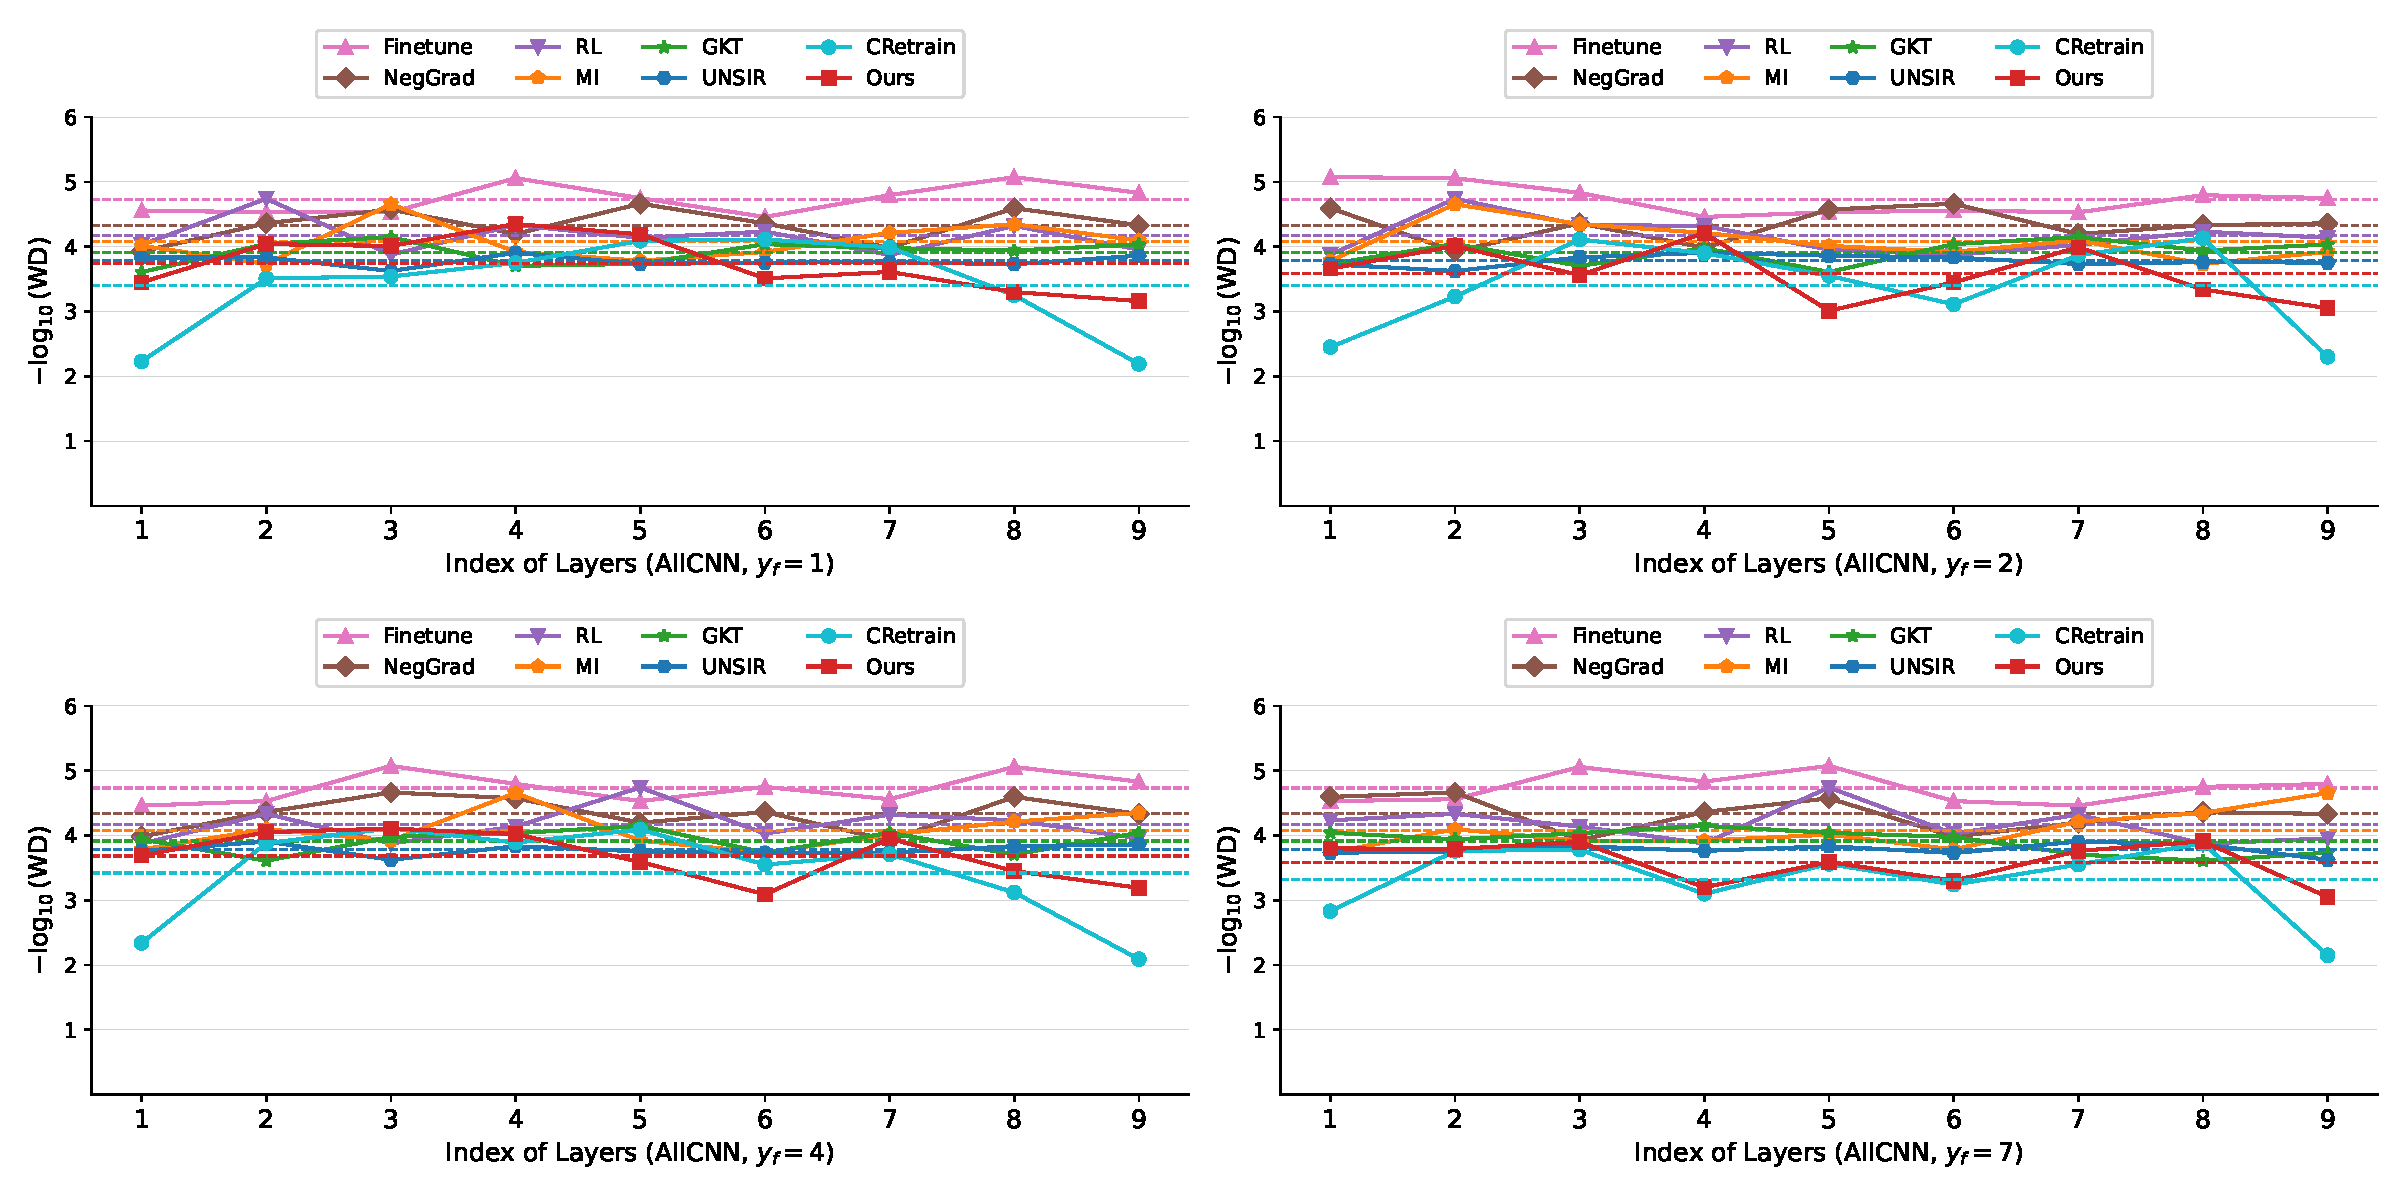
\includegraphics[width=\textwidth]{output1_new.pdf} \\

  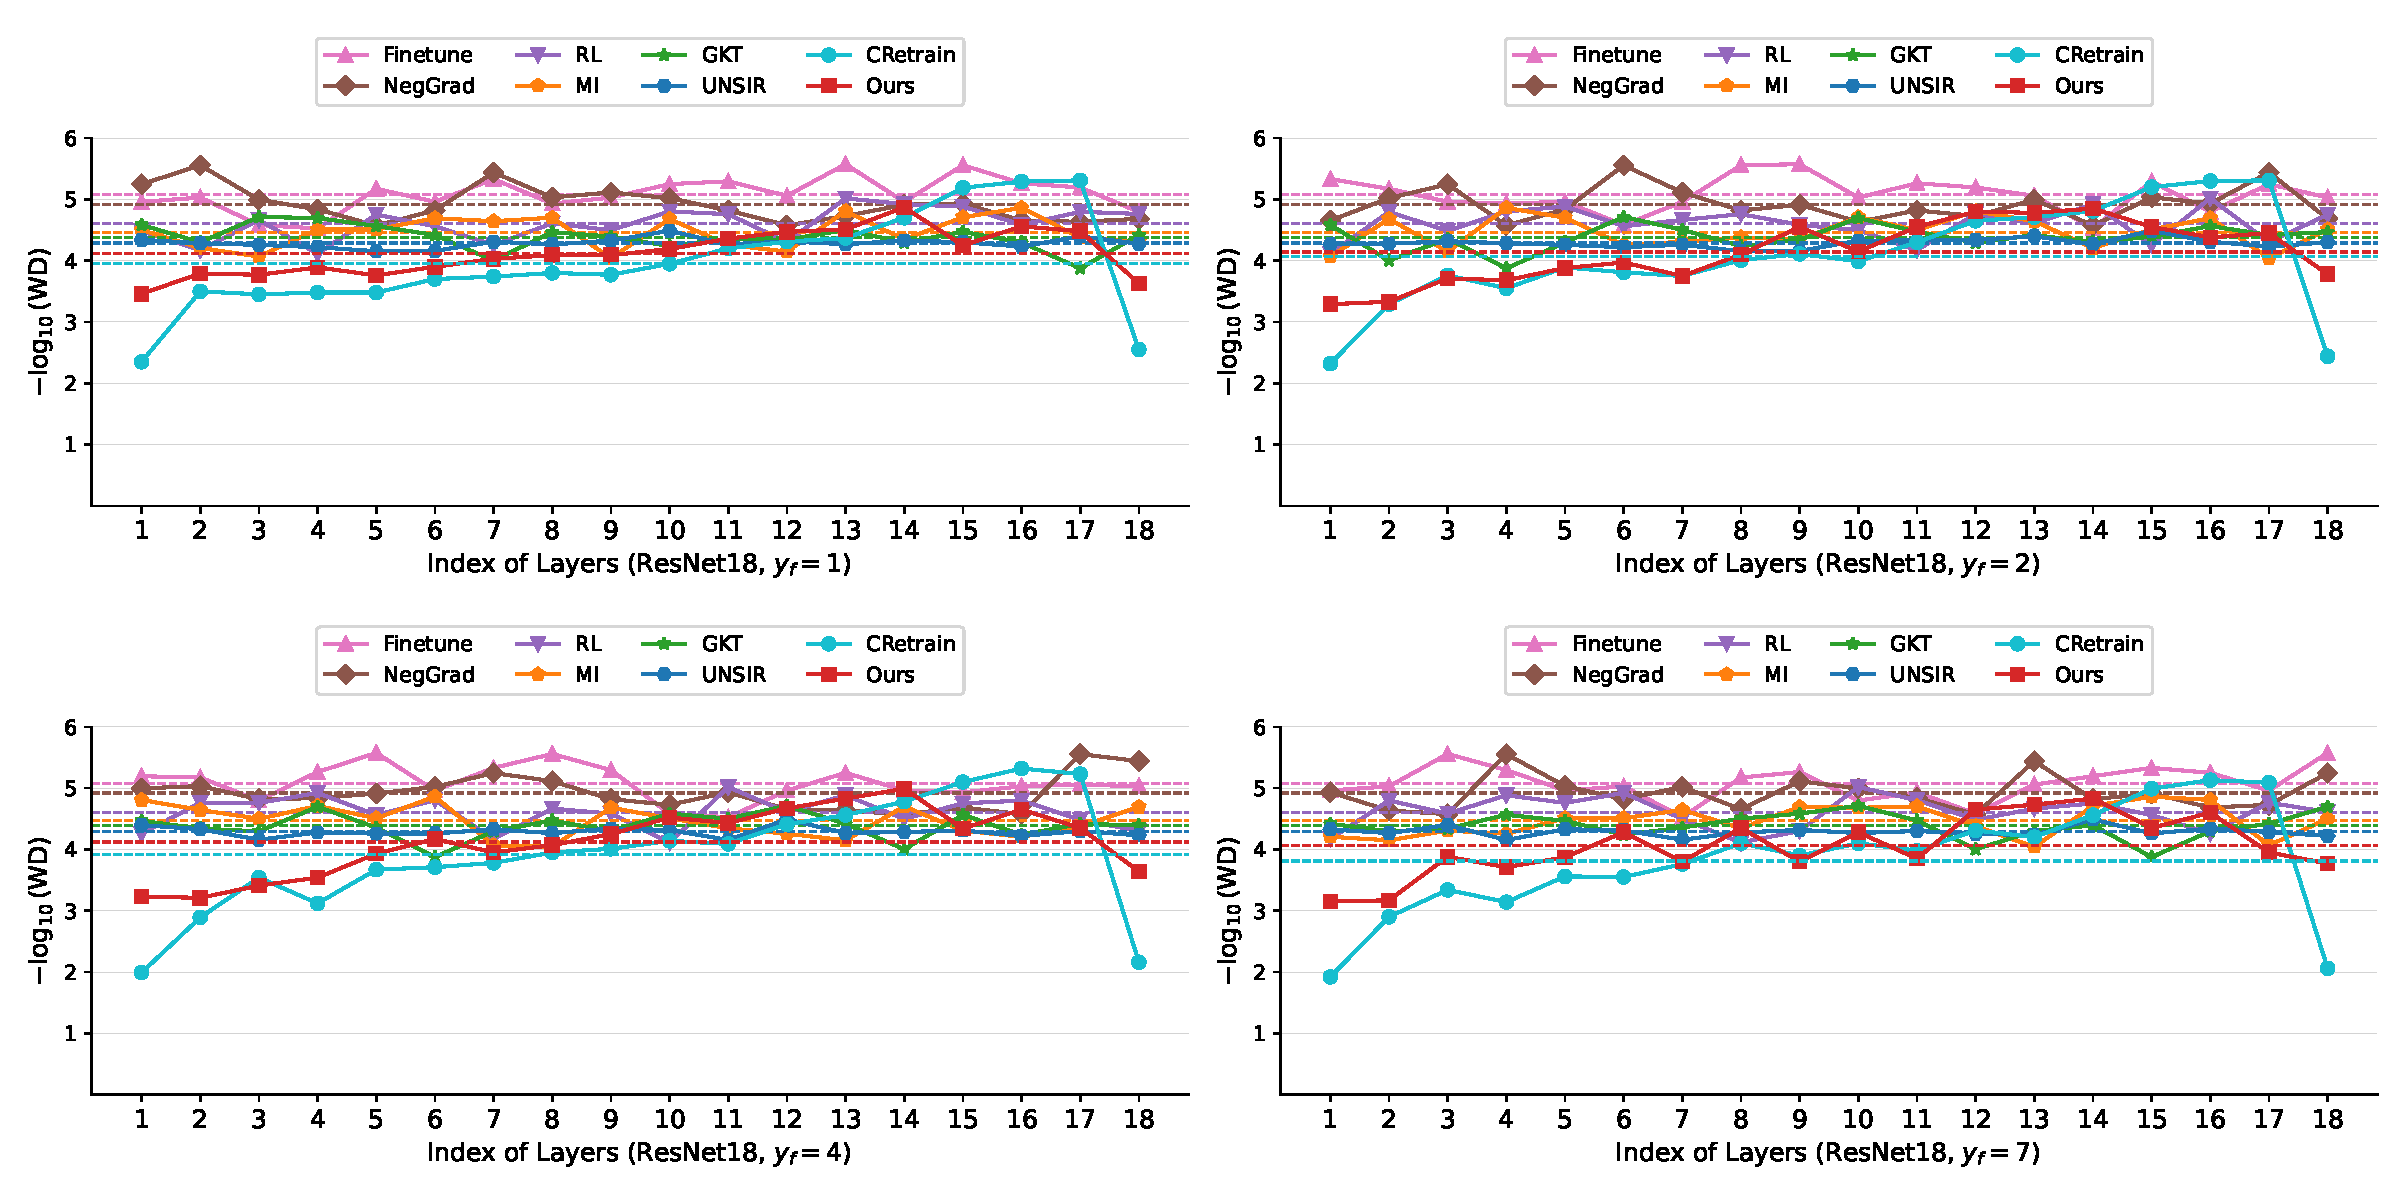
\includegraphics[width=\textwidth]{output2_new.pdf} \\
  \end{tabular}
\end{minipage}

% \caption{Weight Distance ($\textit{WD}$) comparisons across different layers for AllCNN and ResNet18 prediction models on the CIFAR-10 dataset, with varying $\mathcal{Y}_f$ values (1, 2, 4, 7).}
% \caption{Results of Weight Distance ($\textit{WD}$) across different layers of the AllCNN and ResNet18 prediction models on the CIFAR-10 dataset, after applying the CRetrain and our framework, with varying $\mathcal{Y}_f$ values (1, 2, 4, and 7). $\textit{WD}$ is processed by using the negative logarithm, which means that higher values correspond to lower bars in the chart. The dashed lines indicate the average $\textit{WD}$ across all layers for each unlearning method. Notably, our framework yields results comparable to the CRetrain across different predictive models, both showing $\textit{WD}$ in the same order of magnitude and closely aligned metrics, reflecting significant adjustments to the original predictive model parameters made by our framework.}

\caption{Results of Weight Distance ($\textit{WD}$) across different layers of the AllCNN and ResNet18 prediction models on the CIFAR-10 dataset after applying different unlearning methods and our framework, with varying $\mathcal{Y}_f$ values (1, 2, 4, and 7). The $\textit{WD}$ is processed using the negative logarithm, meaning that higher values correspond to lower bars in the chart. The dashed lines indicate the average $\textit{WD}$ across all layers for each unlearning method. Notably, our framework yields results comparable to those of CRetrain across different predictive models, both showing $\textit{WD}$ in the same order of magnitude and closely aligned metrics, reflecting significant adjustments to the original predictive model parameters made by our framework.}


\label{fig_figure3}
\end{figure}


\begin{itemize}
    \item   Accuracy on forget set ($A\mathcal{D}_f$). This metric measures the accuracy of the predictive model in data that need to be forgotten. Ideally, $A\mathcal{D}_f$ should be close to zero, with a lower value indicating better unlearning;
    \item   Accuracy on retain set ($A\mathcal{D}_r$). This metric evaluates the accuracy of the predictive model in retaining data, and should remain close to the accuracy of the original predictive model or higher; 
    \item  Relearn Time (\(RT\)). This metric is used to measure the thoroughness of the unlearning process. Specifically, it represents the minimum number of training epochs required for the predictive model to relearn the forgotten data and recover the original accuracy. In each training epoch, we randomly select 500 samples from the complete training dataset and set the accuracy threshold at 95\%. A higher \(RT\) value indicates better unlearning thoroughness; 
    \item  Weight Distance ($\textit{WD}$). This metric measures the distance between the weights of the original predictive model and the unlearned predictive model at each layer. A higher Weight Distance indicates that the predictive model's weights have been significantly altered, suggesting more thoroughness of the unlearning process. (We use the L2 norm here.)
\end{itemize}


\subsection{GAFN Setting and Unlearning Process}
In our experiments, we configure the generator network \( G \) with a linear layer followed by four transposed convolutional layers. Each transposed convolutional layer is followed by batch normalisation and ReLU activation functions, with the final image output generated by a convolutional layer using a Tanh activation function. In \textit{Maximise} and \textit{Minimise} parts, we set the learning rate to 0.0004 and the weight decay to 1e-4. The predictive model is trained using the Adam optimiser with a batch size of 32 for a total of 100 epochs. During the incremental learning process, we use a Collaborative Training strategy to achieve the purpose of unlearning. The predictive model is trained with a batch size of $32$ using the Adam optimiser at a learning rate of $0.004$ for 1 epoch. Additionally, the Optional Reinforcement Phase strategy is optional; in our experiments, we conduct one round of Optional Reinforcement Phase training with a learning rate set to $0.0004$.

\subsection{Performance Comparison}
\label{subsec_performance_comparison}In our experiments, we compare the proposed framework with the methods in the baselines using the AllCNN and ResNet18 prediction models. The key indicators $A\mathcal{D}_r$, $A\mathcal{D}_f$ and $RT$ in the classification task are shown in Tables 1, 2 and 3 for three different datasets. In addition, in order to measure the thoroughness of the unlearning process, we selecte the commonly used $\textit{WD}$ indicator and conducted experiments on two different models on the CIFAR-10 dataset. The results are shown in Figure 3. We have the following observations:

\begin{itemize}
    \item As shown in Table 1, 2 and 3, our framework achieves an accuracy $A\mathcal{D}_f$ of 0.00\% for all the classes that needed to be forgotten, which is consistent with the performance of CRetrain and indicates successful deletion of the target data. Simultaneously, our framework effectively maintains the predictive accuracy for retain classes, with $A\mathcal{D}_r$ close to that of CRetrain. This demonstrates that the proposed framework preserves the original predictive model's performance while effectively achieving unlearning.

    \item Our framework exhibits consistently excellent performance across different predictive models (AllCNN and ResNet18) and multiple datasets (Fashion MNIST, CIFAR-10, CIFAR-20). Notably, the performance does not degrade with increased network depth or dataset complexity. Furthermore, the proposed framework effectively handles a range of unlearning requirements, from single-class to multi-class forgetting. As a result, our framework has strong scalability and generalizability, adapting well to various unlearning scenarios.

    \item As observed in Figure 3, our framework exhibits $\textit{WD}$ values that are consistent with those obtained using CRetrain, both showing $\textit{WD}$ values in the same order of magnitude and closely aligned metrics. This indicates significant changes in the parameters of each layer post-unlearning. Additionally, the similar large $RT$ value to that of CRetrain suggests that the predictive model requires more epochs to recover the forgotten data. These metrics imply that our framework thoroughly adjusts the predictive model's parameters to achieve unlearning, further confirming the thoroughness of our framework.
\end{itemize}

These detailed observations not only highlight the efficiency and reliability of our framework but also demonstrate its potential advantages in performing precise and comprehensive unlearning tasks. While CRetrain remains the gold standard in scenarios with the complete training dataset, our framework shows unique advantages in other contexts. It maintains high retention accuracy even when data is limited, and in scenarios with strict privacy requirements, it avoids accessing any data to be forgotten which is more compliant with privacy demands. Additionally, our framework is more efficient in handling small or constrained datasets, enabling faster achievement of the desired unlearning.

\subsection{Privacy and robustness}

The purpose of machine unlearning is to efficiently and securely remove the influence of private data from the training dataset in a machine learning model. However, although many algorithms maintain efficiency and security in forgetting private data, they reveal another privacy risk in handling the original dataset. These algorithms often require access to the private data in question, using it as input to execute the unlearning process. This does not comply with the privacy protection principle that sensitive data should remain completely invisible. In machine unlearning, not only do we require the unlearning algorithm to effectively forget private data, but we also insist that, throughout the entire forgetting process, no private data should be accessed.

Our framework is designed from the ground up to ensure that it does not need to access any data requiring unlearning. Additionally, our framework has low requirements regarding the integrity of the original training dataset. In the experimental setup of the previous section, we assume that only 20\% of the dataset, excluding the data to be unlearned, is accessible. Reducing the dataset size means that our unlearning algorithm is more widely applicable and provides stronger privacy protection. This is because the remaining 80\% of the data may involve privacy issues and needs to be unlearned, yet we never need to access, collect, or store this part of the data. Furthermore, we reduced the dataset ratio even further to study our framework's robustness with a smaller sample size. We compared our framework with all the methods mentioned in the previous section, focusing particularly on performance in terms of $A\mathcal{D}_f$ and $A\mathcal{D}_r$, as shown in Figure 4.


\begin{figure}[t]  
    \centering
    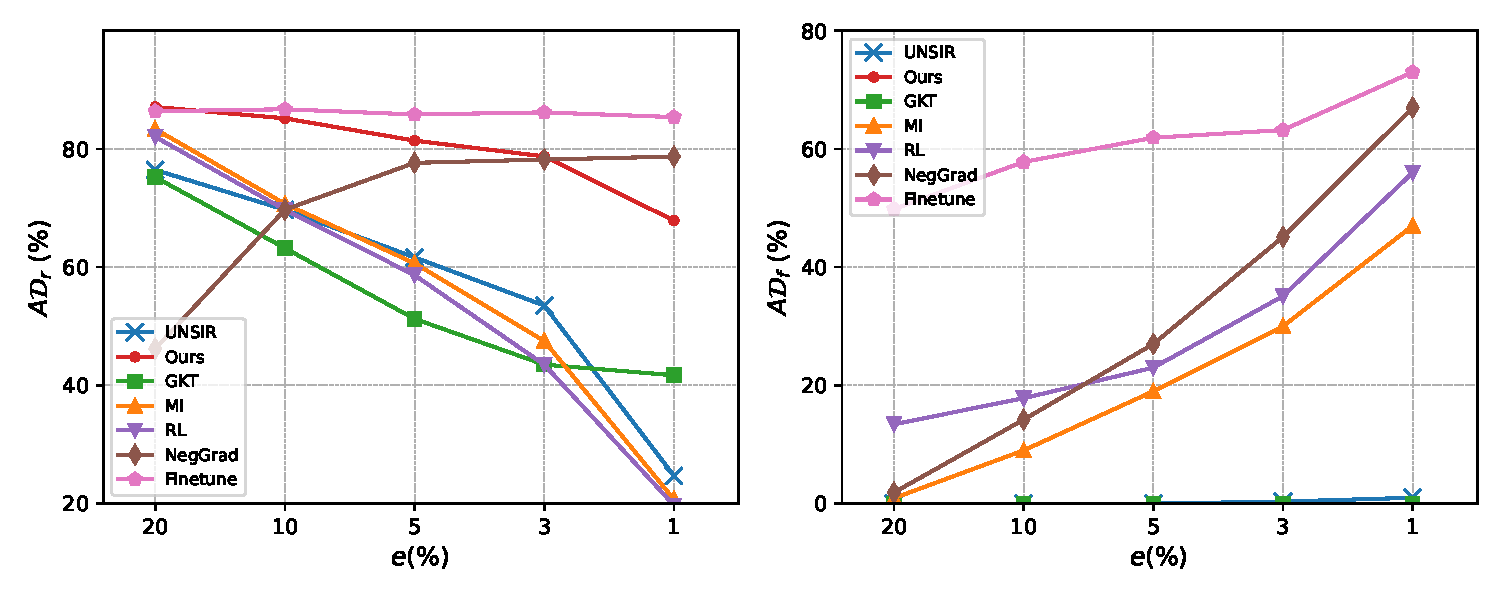
\includegraphics[width=\textwidth]{output4_new.pdf}
    \caption{Comparison of $A\mathcal{D}_r$ (left) and $A\mathcal{D}_f$ (right) values across different sets of \(e\) for mentioned methods and our framework on ResNet18 with CIFAR-10 dataset, using $\#\mathcal{Y}_f$ = 1.}
    \label{fig_figure4}
\end{figure}


As shown in Figure 4, our framework demonstrates outstanding robustness in few-shot scenarios, maintaining high performance even as the available training dataset decreases. The left side of Figure 4 shows a comparison of $A\mathcal{D}_r$ between our framework and other methods for different values of \(e\). The accuracy of the retain classes in our framework remains consistently high, ranging from 67.88\% to 87.10\%. Notably, when the sample ratio exceeds 3\%, $A\mathcal{D}_r$ remains almost unchanged, with only a slight decrease when \(e\) falls below 3\%. In contrast, the $A\mathcal{D}_r$ of UNSIR decreases significantly as the available training data diminishes, with a sharp drop when the dataset is extremely limited (around 1\%), resulting in a gap of up to 43.17\% compared to our framework.

Similar to UNSIR, GKT, MI, and RL also exhibit a severe decline in retained class accuracy as the sample ratio decreases. However, Finetune and NegGrad maintain high accuracy for retain classes, with NegGrad even showing increased accuracy as the sample ratio decreases. This increase, however, does not indicate that they are effective unlearning algorithms, as shown by the high $A\mathcal{D}_f$ values on the right side of Figure 4, which indicate that these methods fail to achieve effective unlearning.

The right side of Figure 4 illustrates the comparison of $A\mathcal{D}_f$. When the proportion of available training data falls below 5\%, UNSIR, GKT, and our framework all achieve close to 0\% $A\mathcal{D}_f$, indicating good unlearning performance for the target classes. In contrast, Finetune, NegGrad, RL, and MI show increasing prediction accuracy for the classes to be unlearned as the sample ratio \(e\) decreases, indicating their lack of effective unlearning capability in few-shot scenarios.

In summary, under stricter conditions with fewer samples, our framework demonstrates the best performance, showcasing strong robustness.


\section{Conclusion}
In this paper, we propose a framework for class unlearning in few-shot scenarios under zero-glance conditions. Our framework leverages generative samples to mitigate the influence of the data to be forgotten, enabling effective unlearning while maintaining model performance. Experimental results demonstrate that our method performs robustly with partial training dataset, thereby enhancing privacy and security in machine learning applications.


 
\section*{Acknowledgements}
The authors would like to thank the efforts from anonymous reviewers.
This work was supported in part by the National Key Research and Development Program of China (2021YFB3101304), in part by the Fundamental Research Funds for the Central Universities of Ministry of Education of China (ZYTS24145, GLZX24039), and in part by the Technology Innovation Leading Program of Shaanxi (2024QCY-KXJ-171).

\bibliographystyle{elsarticle-num} 
\bibliography{ref}

\end{document}

\endinput
%%
%% End of file `elsarticle-template-num.tex'.
